\documentclass[journal]{IEEEtran}

%\usepackage[brazilian]{babel}

\makeatletter
%\adddialect\l@BRAZILIAN\l@brazilian
\makeatother


\usepackage[T1]{fontenc}
\usepackage[utf8]{inputenc}
\usepackage{lmodern}

\usepackage{ae}
\usepackage{hyphenat}
\usepackage{fancyhdr}
\usepackage{float}
\usepackage{cite}
\usepackage[pdftex]{hyperref}
\usepackage[pdftex]{color,graphicx}

\usepackage[cmex10]{amsmath}
\usepackage[]{equations}
\usepackage{array}

\usepackage{mdwmath}
\usepackage{mdwtab}
\usepackage{url}
\usepackage{tikz}

\hyphenation{op-tical net-works semi-conduc-tor con-si-de-ram fa-mi-lia-ri-za-ção}
\hypersetup{colorlinks, citecolor=black, filecolor=black, linkcolor=black, urlcolor=blue}

%Algoritmos
\usepackage[english]{algorithm2e}

\begin{document}
\title{Introduction to Numeric Simulation of Magnetic Fluid Flows}

\author{Ataias~Pereira~Reis, Yuri~Dumaresq~Sobral, Francisco~Ricardo~da~Cunha\\Universidade de Brasília\\Departamento de Matemática\\Brasília, Brasil\\ataiasreis@gmail.com}

% The paper headers
\markboth{Scientific Initiation Program, August~2015}%
{Shell \MakeLowercase{\textit{et al.}}: Bare Demo of IEEEtran.cls for Journals}

\maketitle


\begin{abstract}
%\boldmath
This work aims at studying the behavior of magnetic fluids in a 2D lid-driven cavity. In order to achieve this goal, a computer program was developed to solve the Navier-Stokes equation using finite differences. In addition to that, different equations for the evolution of the magnetism of the magnetic fluid were introduced. The governing equations in continuous form and also in discrete form are presented, as well as the dimensionless parameters governing the problem. The Navier-Stokes equations are solved using a projection method to decouple the velocity pressure problem. The solution of the Poisson equation is obtained by means of an implicit method with sparse matrices and Cholesky factorization. Once the hydrodynamic and magnetostatic parts are solved, vector fields and streamlines are plotted for analysis of the flow. A few distinct Reynolds numbers are tested, as well as some different magnetic parameters. We observe that the magnetic field strongly influences the flow on the cavity.

\end{abstract}
% IEEEtran.cls defaults to using nonbold math in the Abstract.
% This preserves the distinction between vectors and scalars. However,
% if the journal you are submitting to favors bold math in the abstract,
% then you can use LaTeX's standard command \boldmath at the very start
% of the abstract to achieve this. Many IEEE journals frown on math
% in the abstract anyway.

% Note that keywords are not normally used for peerreview papers.
\begin{IEEEkeywords}
Magnetic fluid, Driven Cavity, Finite~differences, Magnetohydrodynamics
\end{IEEEkeywords}

% For peer review papers, you can put extra information on the cover
% page as needed:
% \ifCLASSOPTIONpeerreview
% \begin{center} \bfseries EDICS Category: 3-BBND \end{center}
% \fi
%
% For peerreview papers, this IEEEtran command inserts a page break and
% creates the second title. It will be ignored for other modes.
\IEEEpeerreviewmaketitle

\section{Introduction}
A colloidal magnetic fluid, or ferrofluid, consists typically of a suspension of monodomain ferromagnetic particles such as magnetite in a nonmagnetic carrier fluid. Particle-to-particle agglomeration is avoided by surfactants covering the particles, and Brownian motion prevents particle sedimentation in gravitational or magnetic fields\cite{RosensweigMagneticFluids}. Magnetic fluids have usually around $10^{23}$ magnetic nano-particles per cubic meter and are opaque at visible light since most of them are oil-based.

This project aims at studying magnetic fluids in a 2D lid-driven cavity. The cavity studied in this work is a square. The lid has a stationary velocity and all the boundaries have null velocities. Even though this may seem a simple problem, papers have been presented not only in the last century but also in the current to study real problems: Garandet \cite{Garandet2012149} uses a similar approach to study solute segregations; on the field of biomagnetic fluids, Tzirtzilakis \cite{Tzirtzilakis2013} has also considered a cavity and analyzed the stationary solutions under different conditions of the Reynolds numbers and magnetic parameters. Differently from this last work, our project has not considered a method to find directly the steady-state flow, but has evolved in discrete time steps from rest until the steady state is reached. The advantage is that more data can be analyzed, so that it is possible to know when vortices start to appear and if there are any that disappear during the evolution to steady-state. 

The differential equations governing this problem will be solved using finite differences \cite{zbMATH03010997}, a method that approximates each derivative by discrete terms involving differences. The domain in which the problem is to be solved must be turned into a mesh. The smaller the cells of the mesh, the better the finite differences solution will be. All the finite differences used here are of second order, which means that the error decays quadratically as the number of points in the mesh increases. The mesh that is being used is a staggered grid. 
\section{Governing Equations}
\subsection{Hidrodynamics}
Equations \ref{navierstokes} and \ref{navierincompressibilidade} govern the flow of an incompressible fluid. The first one is the Navier-Stokes equation \cite{batchelor}, while the second one is the condition for incompressibility: \begin{eqnarray}
\left( \frac{\partial {\textbf{v}}}{\partial t}+\textbf{v}\cdot\nabla \textbf{v} \right)=-\nabla p+\frac{1}{\mathit{Re}}\nabla^2 \textbf{v} + \textbf{f}\label{navierstokes},\\
\nabla\cdot\textbf{v}=0.\label{navierincompressibilidade}
\end{eqnarray}

In the latter equations, some terms are presented: $\mathbf{v}$ is the velocity, $p$ stands for pressure and $\mathbf{f}$ is an external force acting on the fluid, which is, in our case, created by a magnetic field. The Reynolds number $\mathit{Re}$ is given by \begin{eqnarray}
\mathit{Re}=\frac{\rho L U}{\mu},
\end{eqnarray} in which $\rho$ is the density of the fluid, $L$ is a characteristic linear dimension, in our case, the size of the cavity, $U$ is maximum speed of the lid and $\mu$ is the dynamic viscosity of the fluid.



A specific solution of the Navier-Stokes equation is found by stating its boundary and initial conditions. For the current work, the boundary conditions are \begin{eqnarray}
u(x,1) & = & \sin^2(\pi x),\label{condition1ns}\\
u(x,0) & = & u(0,y) = u(1,y) = 0,\label{condition2ns}\\
v(x,0) & = & v(x,1) = v(0, y) = v(1, y) = 0\label{condition3ns}
\end{eqnarray} and we start from rest. Note that Equation \ref{condition1ns} was used to prevent corner stress singularities.

\subsection{Magnetism}
Besides the hydrodynamics equations and conditions, the magnetic force $\mathbf{f}$ in Equation \ref{navierstokes} must be computed. From Maxwell's equations, \begin{eqnarray}
\nabla\cdot \mathbf{B} & = & 0\label{secondmagneticequation},
\end{eqnarray} and, for a magnetizable medium, we have \begin{eqnarray}
\mathbf{B} &=& (\mathbf{M}+\mathbf{H}),\label{firstmagneticequation}
\end{eqnarray}
in its dimensionless form. In those equations, $\mathbf{B}$ denotes the magnetic induction, $\mathbf{M}$ the magnetization of the fluid and $\mathbf{H}$ the magnetic field. From the latter equations, it is possible to conclude that \begin{eqnarray}
\nabla\cdot\mathbf{H} = -\nabla\cdot \mathbf{M}\label{mh1}.
\end{eqnarray}

The magnetostatic regime of the Maxwell's equations implies \begin{equation}\nabla\times \mathbf{H} = \mathbf{0},
\end{equation} which indicates there is a potential field $\phi$ that satisfies \begin{equation}\mathbf{H} = -\nabla \phi.\label{Hphipotencial}\end{equation} With these last equations, it is possible to obtain \begin{eqnarray}
\nabla^2\phi &=& \nabla\cdot \mathbf{M}.\label{eqcampomag}
\end{eqnarray}

This is a Poisson equation that will give $\phi$ according the the local magnetization of the ferrofluid. In this work, the superparamagnetic case is being considered, what implies \begin{equation}\mathbf{M} = \chi \mathbf{H}.\end{equation}

Nevertheless, the potential $\phi$ cannot be introduced directly in the Navier-Stokes equation. What is needed is a relation that gives the magnetic force, which could then be incorporated in the fluid equations. The magnetic force is \begin{equation}
	\mathbf{f} = \mathrm{C}_{\mathrm{pm}}\; \mathbf{M}\cdot \nabla \mathbf{H},\label{magneticforce}\end{equation} in which $\mathrm{C}_{\mathrm{pm}}$, the magnetic pressure coefficient for the superparamagnetic case, is \begin{eqnarray}
\mathrm{C}_{\mathrm{pm}} & = & \frac{\mu_0 H_0^2}{\rho u^2},\label{cpm}
\end{eqnarray} in which $H_0$ is the characteristic magnetic field scale and equals $\gamma$ in Equations \ref{Hx} and \ref{Hy}.

The boundary conditions were not yet determined for the potential field $\phi$. To derive those conditions, an applied magnetic field $\mathbf{H}$ was considered and the requirement of continuity of normal components of the magnetic induction $\mathbf{B}$ accross the boundaries, Equation \ref{firstmagneticequation}. This continuity can be mathematically represented by \begin{equation}\left(\mathbf{B}_{\mathrm{out}} - \mathbf{B}_{\mathrm{in}}\right)\cdot \mathbf{n} = 0 \label{normalconditionB}.\end{equation} 

From Equations \ref{firstmagneticequation} and \ref{normalconditionB}, we have \begin{eqnarray}
(H_{\mathrm{out}}^{\mathrm{n}} + M_{\mathrm{out}}^{\mathrm{n}}) &=&  (H_{\mathrm{in}}^{\mathrm{n}}+M_{\mathrm{in}}^{\mathrm{n}}).\label{normalConditionB2}
\end{eqnarray}

The medium outside is air and therefore its magnetization $M_{\mathrm{out}}^{\mathrm{n}}$ is zero. The term $H_{\mathrm{out}}^{\mathrm{n}}$ is substituted following  Equation \ref{Hphipotencial}, resulting  in: \begin{eqnarray}
\nabla\phi_{\mathrm{d}}^{\mathrm{n}} & = & -H_{\mathrm{out}}^{\mathrm{n}} + M_{\mathrm{in}}^{\mathrm{n}}. \label{nablaphid}
\end{eqnarray}

From that, four Neumann boundary conditions can be obtained for Equation \ref{eqcampomag}: \begin{eqnarray}
\left.\frac{\partial \phi}{\partial x}\right|_{x=0} &\approx& -H^{x}_{2,j} + M^{x}_{2,j}\label{condition1phi},\\
\left.\frac{\partial \phi}{\partial x}\right|_{x=1} &\approx& -H^{x}_{n,j} + M^{x}_{n,j},\\
\left.\frac{\partial \phi}{\partial y}\right|_{y=0} &\approx& -H^{y}_{i,2} + M^{y}_{i,2},\\
\left.\frac{\partial \phi}{\partial y}\right|_{y=1} &\approx& -H^{y}_{i,n} + M^{y}_{i,n};\label{condition4phi}
\end{eqnarray} in which the subscripts are indicating matrix indices.

\section{Numerical Solution of the Governing Equations}

\subsection{Grid configuration}

As stated before, an staggered-grid is used to eliminate spurious pressure modes. In such a grid, not every information is stored in the same point. For instance, on the cell $ij$, the pressure will be in position $i+\frac{1}{2}j+\frac{1}{2}$, while velocity in the $x$ direction will be $u_{ij+\frac{1}{2}}$ and the $y$ direction will be $v_{i+\frac{1}{2}j}$. This avoids spurious pressure modes as described in \cite{hinchLectureNotes}. A cell of this grid is presented in Figure \ref{grid-cell}, while the mesh is presented in Figure \ref{staggered-grid}. After the solution is obtained, an interpolation can be made to obtain the values at any specified point. We have chosen to plot all the results in the middle point of each cell. The pressure is already in that position, but the velocities are not. Therefore, averages were computed to obtain those values in the middle point. The discretizations of the following sections all consider a staggered-grid.

\begin{figure}[!ht]
\centering
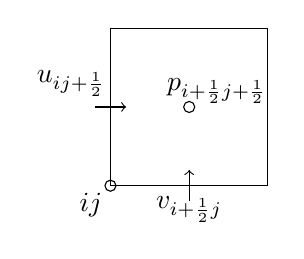
\begin{tikzpicture}
\draw (0,0) rectangle (2,2);
\draw (1.35,1.2) node {$p_{i+\frac{1}{2}j+\frac{1}{2}}$};
\draw[->] (1,-0.2) -- (1,0.2);
\draw (1,-0.3) node {$v_{i+\frac{1}{2}j}$};
\draw[->] (-0.2,1) -- (0.2,1);
\draw (-0.5,1.3) node {$u_{ij+\frac{1}{2}}$};
\draw (1,1) circle (2pt);

\draw (0,0) circle (2pt);
\draw (-0.25,-0.25) node {$ij$};
\end{tikzpicture}
\caption{Cell of the staggered grid\label{grid-cell}}
\end{figure}

\begin{figure}[!ht]
\centering
\tikzstyle{help lines}+=[dashed]
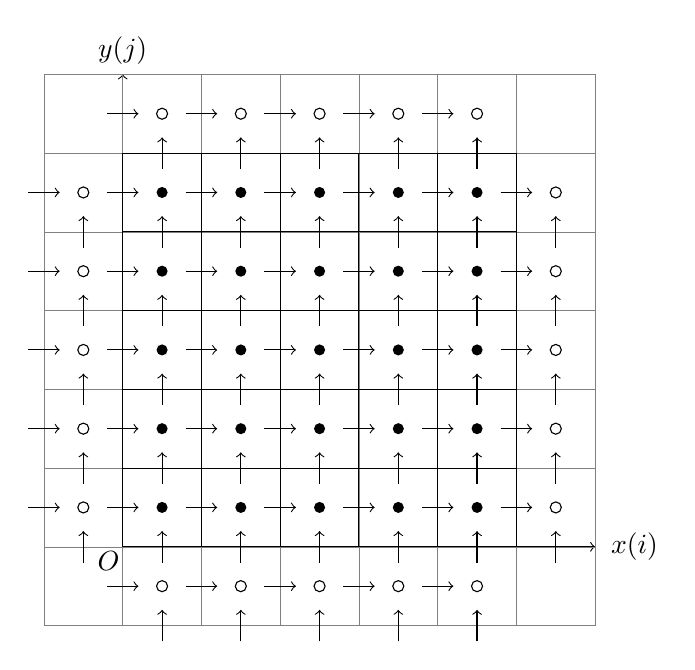
\begin{tikzpicture}
%axes
\draw[->] (0,5) -- (xyz cs:y=6);
\draw (0,6.3) node {$y(j)$};
\draw[->] (5,0) -- (xyz cs:x=6);
\draw (6.5,0) node {$x(i)$};
\draw (-0.18,-0.18) node {$O$};
%grid
\draw[style=help lines] (-1,-1) grid +(7,7);
\draw (0,0) grid +(5,5);
%internal p points
\foreach \x in {0.5,1.5,2.5,3.5,4.5}
  \foreach \y in {0.5,1.5,2.5,3.5,4.5}
  {
  \fill (canvas cs:x=\x cm,y=\y cm) circle (2pt);
}
%External p points
\foreach \x in {0.5,1.5,2.5,3.5,4.5}
  \draw (\x,-0.5) circle (2pt);
\foreach \y in {0.5,1.5,2.5,3.5,4.5}
  \draw (5.5,\y) circle (2pt);
\foreach \y in {0.5,1.5,2.5,3.5,4.5}
  \draw (-0.5,\y) circle (2pt);
\foreach \x in {0.5,1.5,2.5,3.5,4.5}
  \draw (\x,5.5) circle (2pt);
%Internal Horizontal Velocities Points
\foreach \x in {-1.2,-0.2,0.8,1.8,2.8,3.8,4.8}
  \foreach \y in {0.5,1.5,2.5,3.5,4.5}
  {
  \draw[->] (\x,\y) -- (\x+0.4,\y);
}
%External Horizontal Velocities Points
\foreach \x in {-.2,0.8,1.8,2.8,3.8}
  \draw[->] (\x,5.5) -- (\x+0.4,5.5);
\foreach \x in {-.2,0.8,1.8,2.8,3.8}
  \draw[->] (\x,-.5) -- (\x+0.4,-.5);
%Internal Vertical Velocities Points
\foreach \x in {0.5,1.5,2.5,3.5,4.5}
  \foreach \y in {-1.2,-0.2,0.8,1.8,2.8,3.8,4.8}
  {
  \draw[->] (\x,\y) -- (\x,\y+0.4);
}
%External Vertical Velocities Points
\foreach \y in {-0.2,0.8,1.8,2.8,3.8}
  \draw[->] (5.5,\y) -- (5.5,\y+0.4);
\foreach \y in {-0.2,0.8,1.8,2.8,3.8}
  \draw[->] (-.5,\y) -- (-.5,\y+0.4);
\end{tikzpicture}
\caption{Staggered-grid. Dark circles are internal points, while empty ones are part of the extra layer\label{staggered-grid}}
\end{figure}

The code for the simulator was made with aid of programming language Julia, more information about this language is available at \cite{JuliaProgramming}. Julia offers several linear algebra packages that are easy to use and very efficient. Graphics were made using Python's graphical packages \cite{matplotlib}. Codes and articles of this project are hosted on GitHub\cite{gitHubFerrofluidos}.


\subsection{Time-splitting}
In order to discretize the Navier-Stokes equation, an expansion is performed in directions $x$ and $y$ to obtain scalar equations: \begin{eqnarray}
\frac{\partial u}{\partial t}+u\frac{\partial u}{\partial x}+v\frac{\partial
u}{\partial y}=-\frac{\partial p}{\partial
x}+\frac{1}{\mathit{Re}}\left(\frac{\partial^2 u}{\partial^2 x}+\frac{\partial^2 u}{\partial^2
y}\right)+f_x, \label{navierX}\\
\frac{\partial v}{\partial t}+u\frac{\partial v}{\partial x}+v\frac{\partial
v}{\partial y}=-\frac{\partial p}{\partial
y}+\frac{1}{\mathit{Re}}\left(\frac{\partial^2 v}{\partial^2 x}+\frac{\partial^2 v}{\partial^2
y}\right)+f_y. \label{navierY}
\end{eqnarray} 

Finite differences of second order need to be applied to discretize Equations \ref{navierX} and \ref{navierY}. Nevertheless, a naive application of the discretized formulas will not yield a proper solution, as the fluid flow equation is highly non-linear due to its convective term $\mathbf{v}\cdot \nabla \mathbf{v}$. Also, pressure is not known in advance so, while it is needed at each time step, it is also an unknown that must be found. A method developed by Chorin, named time-splitting, and described in \cite{Chorin1997118} was used to resolve this problem. Firstly, one starts by applying finite differences for the velocity derivative with respect to time and then manipulating by summing and subtracting an arbitrary quantity $\mathbf{v}^*$ in the numerator, as in \begin{equation}
\frac{\partial \textbf{v}}{\partial t}\approx \frac{\textbf{v}^{n+1}-\textbf{v}^n}{\Delta t}=\frac{\textbf{v}^{n+1}-\textbf{v}^*}{\Delta t}+\frac{\textbf{v}^{*}-\textbf{v}^n}{\Delta t}, \label{vdottimesplitting}
\end{equation} in which $\mathbf{v}^n$ is the velocity at the current time-step and $\mathbf{v}^{n+1}$ is the velocity one time-step in the future.

The aforementioned technique imposes on the first term of the right hand side of Equation \ref{vdottimesplitting} a relation with the pressure field: 
\begin{equation}\frac{\textbf{v}^{n+1}-\textbf{v}^*}{\Delta t}=-\nabla p\label{equacaoprepressao}.\end{equation}

Note that Equation \ref{equacaoprepressao} already shows a relation between $\mathbf{v}^{n+1}$ and $\mathbf{v}^{*}$, a correlation that is pertinent because it is used to obtain the velocity in the next time step after pressure is calculated.


The second term on the RHS of Equation \ref{vdottimesplitting} is responsible for all the terms of Equation \ref{navierstokes}, except the pressure gradient term that is already considered on Equation \ref{equacaoprepressao}: \begin{eqnarray}
\frac{\textbf{v}^{*}-\textbf{v}^n}{\Delta t}&=& \frac{1}{\mathit{Re}}\nabla ^2 \textbf{v} + \textbf{f} - \textbf{v}\cdot \nabla \textbf{v}\label{equacaovestrela}
\end{eqnarray}

The term $\mathbf{v}^*$ can be isolated in Equation \ref{equacaovestrela} and then calculated easily as only known terms from time step $n$ are involved in the aforementioned equation. Nevertheless, only time was discretized so far. Before any computation, we need to apply finite differences to Equation \ref{equacaovestrela}, which results in %------------------- u* -------------------
\begin{eqnarray}
u_{ij}^{*}&=&u_{ij}^n+\Delta t\left[\frac{1}{\mathit{Re}}\left(\frac{u_{ij}^s-4u_{ij}^n}{\Delta
x^2}\right)+Fx_{ij}^n\right] + \nonumber \\
&-&\left[u_{ij}^n(u_{i+1j}^n-u_{i-1j}^n)+ \right.\nonumber \\
&+& \left. v_{ij}^t(u_{ij+1}^n-u_{ij-1}^n)\right]\frac{\Delta t}{2\Delta x}\; \textrm{and }\label{step1-3}
\end{eqnarray}
%------------------- v* ------------------
\begin{eqnarray}
v_{ij}^{*}&=&v_{ij}+\Delta t\left[\frac{1}{\mathit{Re}}\left(\frac{v_{ij}^s-4v_{ij}^n}{\Delta
x^2}\right)+Fy_{ij}^n\right] \nonumber \\
&-&\left[u_{ij}^t (v_{i+1j}^n-v_{i-1j}^n)+ \right.\nonumber \\
&+& \left. v_{ij}^n(v_{ij+1}^n-v_{ij-1}^n)\right]\frac{\Delta t}{2\Delta x}.\label{step1-4}
\end{eqnarray}

In the latter equations, $u^*_{ij}$ is a velocity in the $x$-direction at row $i$ and column $j$ in the mesh, while $v^*_{ij}$ is a velocity in the $y$-direction with similar indexing. It is important to notice that those equations have truncated the $1/2$ that would appear when the value is stored in the middle of the cell, or at the middle of a wall. In order to the computations to be valid, the values involved must be related to the same physical point. The terms $u_{ij}^t$ and $v_{ij}^t$ are interpolated velocities that need to be defined in order for the computations to be correct in the staggered-grid and are defined as: \begin{eqnarray}
u_{ij}^t&=&\frac{1}{4}(u_{ij}^n+u_{i+1j}^n+u_{i+1j-1}^n+u_{ij-1}^n) \label{ut},\\ 
v_{ij}^t &=& \frac{1}{4}(v_{ij}^n+v_{i-1j}^n+v_{i-1j+1}^n+v_{ij+1}^n). \label{vt}
\end{eqnarray}

The terms $u^s_{ij}$ and $v^s_{ij}$ refer to a sum of cell points around the corresponding velocity located in $ij$: \begin{eqnarray}
u_{ij}^s &=& \SumFour{u} \label{us}, \\
v_{ij}^s &=& \SumFour{v} \label{vs}.
\end{eqnarray}

As a means to calculate $p$, the divergence operator is applied to both sides of Equation \ref{equacaoprepressao}: \begin{eqnarray}
	-\nabla\cdot\nabla p & = &\nabla\cdot \left(\frac{\textbf{v}^{n+1}-\textbf{v}^*}{\Delta t}\right).
\end{eqnarray}

As $\mathbf{v}^{n+1}$ has to obey the incompressibility condition, its divergence is zero, with the remaining equation being transformed into a Poisson equation: \begin{eqnarray}
\nabla^2 p & = & \frac{1}{\Delta t}\nabla\cdot \textbf{v}^{*}.	 \label{pressureVStar}
\end{eqnarray}



In order to solve Equation \ref{pressureVStar}, its boundary conditions need to be determined. Equations \ref{navierX} and \ref{navierY} are valid in the whole domain, including the walls. To obtain the boundary conditions for $p$, these equations are evaluated according to Equations \ref{condition1ns} to \ref{condition3ns}, which results in:\begin{eqnarray} \frac{\partial p}{\partial x}\Bigg|_{\textrm{wall}}&=&\frac{1}{\mathit{Re}}\frac{\partial^2
u}{\partial x^2}\Bigg|_{\textrm{wall}}+f_x,\label{paredesVerticais}\\
\frac{\partial p}{\partial y}\Bigg|_{\textrm{wall}}&=&\frac{1}{\mathit{Re}}\frac{\partial^2
v}{\partial y^2}\Bigg|_{\textrm{wall}}+f_y.\label{paredesHorizontais}
\end{eqnarray}

Equation \ref{paredesVerticais} gives conditions for the left and right boundaries, while Equation \ref{paredesHorizontais} is for top and bottom. As the four walls have flux conditions, Neumann conditions, there are infinitely many solutions that differ only by a constant. Therefore, a point in the mesh is specified arbitrarily so that the program converges to a specific solution. This is allowed in our problem, as pressure itself is not directly needed, but only its gradient.

At this stage, $\mathbf{v}^*$ and $p$ are known, so that $\mathbf{v}^{n+1}$ can be calculated by \begin{eqnarray}
	\mathbf{v}^{n+1} & = & \mathbf{v}^*  - \Delta t\cdot  \nabla p. \label{nextStepV}
\end{eqnarray}

Equation \ref{nextStepV} is then used to evolve the system from time $n \Delta t$ to $(n+1)\Delta t$. 

Computer solutions require certain conditions on the time step,$\Delta t$, and spacing of grid points. As well described on \cite{hinchLectureNotes}, the requirements are: stable diffusion, 
\begin{equation}
\Delta t < \frac{1}{4}\mathit{Re}\Delta x^2, \label{stablediffusion}
\end{equation} stable advection, the CFL condition,
\begin{equation}
\Delta t < \frac{\Delta x}{U}, \label{stableadvection}
\end{equation}

 and to resolve well the hydrodynamic boundary layer,  
 \begin{eqnarray}
\Delta x &<& \frac{1}{\mathit{Re}}. \label{boundarylayer}
\end{eqnarray} 

If the time-stepping conditions are not satisfied, the routine will try to solve the flow faster than the laws of physics allow. The result is an incorrect solution or divergency of the solution.


\subsection{Poisson equations}

A pressure must be found that satisfies Equation \ref{pressureVStar}, which is a Poisson equation. The approach to that will be, again, finite differences, but following an implicit approach. Codes that implement explicit difference equations were tested against the implicit ones with the result being that the implicit is much faster. For the implicit case, a linear system must be formed from the difference equations and then the system must be solved to find the pressure. This means that matrix $A$ and vector $b$ must be determined and then system $Ax = b$ must be solved to find $x$ which, in our case, contains pressure values. This system gets very large, but most of the elements in matrix $A$ are 0, so $A$ is a sparse matrix. 

\begin{figure}[!ht]
\centering
\tikzstyle{help lines}+=[dashed]% 
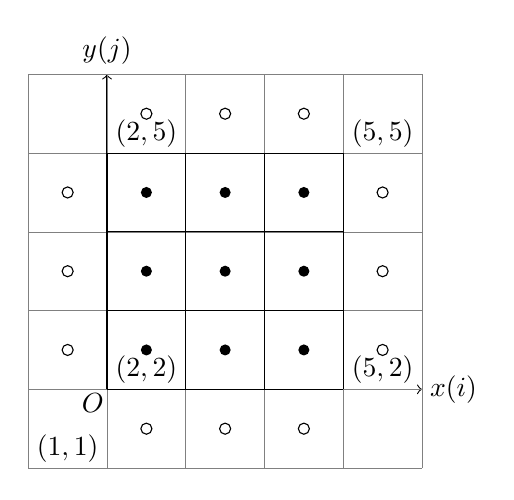
\begin{tikzpicture}
%axes
\draw[->] (0,3) -- (xyz cs:y=4);
\draw (0,4.3) node {$y(j)$};
\draw[->] (3,0) -- (xyz cs:x=4);
\draw (4.4,0) node {$x(i)$};
\draw (-0.18,-0.18) node {$O$};
\draw (-0.5,-0.75) node {$(1,1)$};
\draw (0.5,0.25) node {$(2,2)$};
\draw (3.5,3.25) node {$(5,5)$};
\draw (0.5,3.25) node {$(2,5)$};
\draw (3.5,0.25) node {$(5,2)$};

%grid
\draw[style=help lines] (-1,-1) grid +(5,5);
\draw (0,0) grid +(3,3);
%internal p points
\foreach \x in {0.5,1.5,2.5}
  \foreach \y in {0.5,1.5,2.5}
  {
  \fill (canvas cs:x=\x cm,y=\y cm) circle (2pt);
}
%External p points
\foreach \x in {0.5,1.5,2.5}
  \draw (\x,-0.5) circle (2pt);
\foreach \y in {0.5,1.5,2.5}
  \draw (3.5,\y) circle (2pt);
\foreach \y in {0.5,1.5,2.5}
  \draw (-0.5,\y) circle (2pt);
\foreach \x in {0.5,1.5,2.5}
  \draw (\x,3.5) circle (2pt);

\end{tikzpicture} 
\caption{Example grid to solve for pressure\label{examplePressureGrid}}
\end{figure}

Obtaining $A$ and $b$ can be done by first analyzing a small grid and then generalizing the result for an $n\times n$ grid. First, a $5\times 5$ grid was considered, as presented in Figure \ref{examplePressureGrid}. The equation to be solved is \begin{equation}
\nabla^2 p = \frac{\partial^2 p}{\partial x^2} + \frac{\partial^2 p}{\partial y^2} = g(x,y), \label{poissonEquation}
\end{equation} in which $g(x,y)$ is any known function of $x$ and $y$. Applying second order central differences to this equation results in \begin{eqnarray}
\frac{p_{i-1j} - 2p_{ij} + p_{i+1j}}{\Delta x^2}	+ \frac{p_{ij-1} - 2p_{ij} + p_{ij+1}}{\Delta x^2} = g_{ij},\label{poissonSecond}
\end{eqnarray} which is a valid equation for internal points (the black dots in Figure \ref{examplePressureGrid}). Isolating term $p_{ij}$ from it results in an explicit equation for the internal points. Explicit equations for the external points are obtained from their boundary conditions. Nevertheless, what is needed is an implicit representation of the system. For that, all the equations, without isolating terms, need to be considered and then organized in matrix form, like \begin{eqnarray}
-4p_{22} + p_{32} + \boldsymbol{p_{12}} + p_{23} + \boldsymbol{p_{21}} &=& \Delta x^2 g_{22}, \label{internalPoissonEq1}\\
-4p_{23} + p_{33} + \boldsymbol{p_{13}} + p_{24} + p_{22} &=& \Delta x^2 g_{23}\label{internalPoissonEq2},\\
-4p_{24} + p_{34} + \boldsymbol{p_{14}} + \boldsymbol{p_{25}} + p_{23} &=& \Delta x^2 g_{24}.\label{internalPoissonEq3}
\end{eqnarray}

The latter equations are three of nine equations that are needed for the internal points of the grid. The rest of the equations can be obtained similarly. Boundary points are marked in bold and equations for them come exactly from boundary conditions. There are twelve external points, what requires the same number of equations, summing up to a total of 21 equations in a $5\times 5$ grid. The four corner points are not taken into account, as they are not used in the grid style adopted, what justifies that only 21 points are used of 25. Equations \ref{pressureBoundary1} to \ref{pressureBoundary4} can have its indices substituted in order to get the 12 equations for the boundary points: \begin{eqnarray}
\frac{\partial p}{\partial x}\left(0, y\right) &=& p_x\left(0, y\right)  \approx  \frac{(p_{2j} - p_{1j})}{\Delta x} \label{pressureBoundary1},\\
\frac{\partial p}{\partial x}\left(1, y\right) &=& p_x\left(1, y\right)  \approx  \frac{(u_{5j} - u_{4j})}{\Delta x},\\
\frac{\partial p}{\partial y}\left(x, 0\right) &=& p_y\left(x, 0\right)  \approx \frac{(p_{i2} - p_{i1})}{\Delta x},\\
\frac{\partial p}{\partial y}\left(x, 0\right) &=& u_y\left(x, 0\right)  \approx  \frac{(p_{i5} - p_{i4})}{\Delta x}.\label{pressureBoundary4}
\end{eqnarray}

Arranging appropriately the 21 equations obtained, $A=$\begin{equation}
\left[\begin{array}{ccccccccc}
-2 & 1 & 0 & 1 & 0 & 0 & 0 & 0 & 0\\
1 & -3 & 1 & 0 & 1 & 0 & 0 & 0 & 0\\
0 & 1 & -2 & 0 & 0 & 1 & 0 & 0 & 0\\
1 & 0 & 0 & -3 & 1 & 0 & 1 & 0 & 0\\
0 & 1 & 0 & 1 & -4 & 1 & 0 & 1 & 0\\
0 & 0 & 1 & 0 & 1 & -3 & 0 & 0 & 1\\
0 & 0 & 0 & 1 & 0 & 0 & -2 & 1 & 0\\
0 & 0 & 0 & 0 & 1 & 0 & 1 & -3 & 1\\
0 & 0 & 0 & 0 & 0 & 1 & 0 & 1 & -2 
\end{array}\right]
\end{equation} and $b=$ \begin{eqnarray}
\Delta x\left[\begin{array}{c}
p_x\left(0, \frac{\Delta x}{2}\right) + p_y\left(\frac{\Delta x}{2},0\right)\\
u_x\left(0, \frac{3\Delta x}{2}\right)\\
p_x\left(0, \frac{5\Delta x}{2}\right) - p_y\left(\frac{\Delta x}{2},1\right)\\
p_y\left(\frac{3\Delta x}{2},0\right)\\
0 \\
-p_y\left(\frac{3\Delta x}{2},1\right)\\
-p_x\left(1, \frac{\Delta x}{2}\right) + p_y\left(\frac{5\Delta x}{2},0\right)\\
-u_x\left(1, \frac{3\Delta x}{2}\right)\\
-p_x\left(1, \frac{5\Delta x}{2}\right) - p_y\left(\frac{5\Delta x}{2}, 1\right)
\end{array}\right] + \Delta x^2 \left[\begin{array}{c}
g_{22} \\ g_{23} \\ g_{24} \\ g_{32} \\ g_{33} \\ g_{34} \\ g_{42} \\ g_{43}  \\ g_{44}\end{array}\right]. \label{bPartnulleigen}
\end{eqnarray}

Even though $A$ and $b$ were obtained, one of the Eigenvalues of this system is zero, so the matrix $A$ is not invertible. The reason for that is related to the fact that there are only Neumann boundary conditions and there are infinitely many solutions that differ only by a constant. To solve this problem, one value of the mesh must be specified and the cell to be chosen can be any but one of the corner points, as they don't play any role on the equations. For our problem, $p_{12} = 0$ was chosen, what results in the update of one element of the matrix and one element of the vector: \begin{eqnarray}
A[1,1] &=& -3 \label{aupdate}, \\
b[1] & = & p_y\left(\frac{\Delta x}{2},0\right)\Delta x + \Delta x^2 g_{22}. \label{bupdate}
\end{eqnarray}

A generic relation to obtain $A$ and $b$ grids bigger than $5\times 5$ is not hard to obtain. After coding a routine to generate $A$ and $b$ according to $g(x,y)$ and $n$, a sparse matrix solver like the one available in Julia\cite{JuliaProgramming} is used to obtain $x$. Julia has a package that uses Cholesky factorization to solve the system by just typing \texttt{x = A\textbackslash b}. Nevertheless, this factorizes the matrix every time this line is executed. As matrix $A$ is fixed, the factorization can be done only once and saved in a variable. After that, only the fatorized matrix is used as in \texttt{x = Afactorized\textbackslash  b}, what is a performance-wise decision.

The magnetism equations must be discretized according to second order finite differences as in this section. The Poisson routine obtained in this section is also used to obtain the potential field $\phi$, Equation \ref{eqcampomag}. The discrete formulas are not presented here, but they can be found in the code available on GitHub.



\section{Results}

It is important to validate the code. As part of the solution method, tests of the Poisson routine and of the discretization of the Navier-Stokes equation are made. The Poisson test is to check the error when comparing a computed result with the actual analytical function that solves the PDE. The second test applies to the Navier-Stokes equation and also for the Poisson one: verifying how the error decays according to an increase in mesh size. As all the discrete formulas used are of second order, this error should decay quadratically. The Results section will present both of these tests. Also, Navier-Stokes with magnetism will be tested to check the order of the discretization. Animations were made in order to better examine those results. The code to generate those is written in Python and is available at the GitHub repository \cite{gitHubFerrofluidos}.


\subsection{Validation of the Poisson Solver}

The implementation of the solver was evaluated by testing a few different problems, but only a succinct presentation is done here with one problem: \begin{eqnarray}
\left\{\begin{array}{ccl}
\nabla^2u(x,y) & = & 0,\\
u_x(1,y) & = & \cos 2\pi y,\\
u_n(x,y) & = & 0, \textrm{otherwise, on the boundary}.
\end{array}\right. \label{poissonTest1}
\end{eqnarray}

Its analytical solution is:

\begin{eqnarray}
u(x,y) & = & \frac{\cosh 2\pi x}{2\pi \sinh 2\pi}\cos 2 \pi y .\label{solutionPoissonTest1}
\end{eqnarray}


The Poisson validation routine returns the middle point difference on the grid that was found, this value is then divided by the real value on that point and multiplied by 100 to get a percentage. The maximum grid size used was $320\times 320$. This one had an error smaller than $0.05\%$. The results for different grid sizes are presented in Figure \ref{errorPoissonTest}. It is easy to see that the error decays quadratically, what was expected due to the second order finite differences that were used.



\begin{eqnarray}
u(x,y) & = & \frac{\cosh 2\pi x}{2\pi \sinh 2\pi}\cos 2 \pi y \label{solutionPoissonTest1}
\end{eqnarray}

\begin{figure}[!ht]
\centering
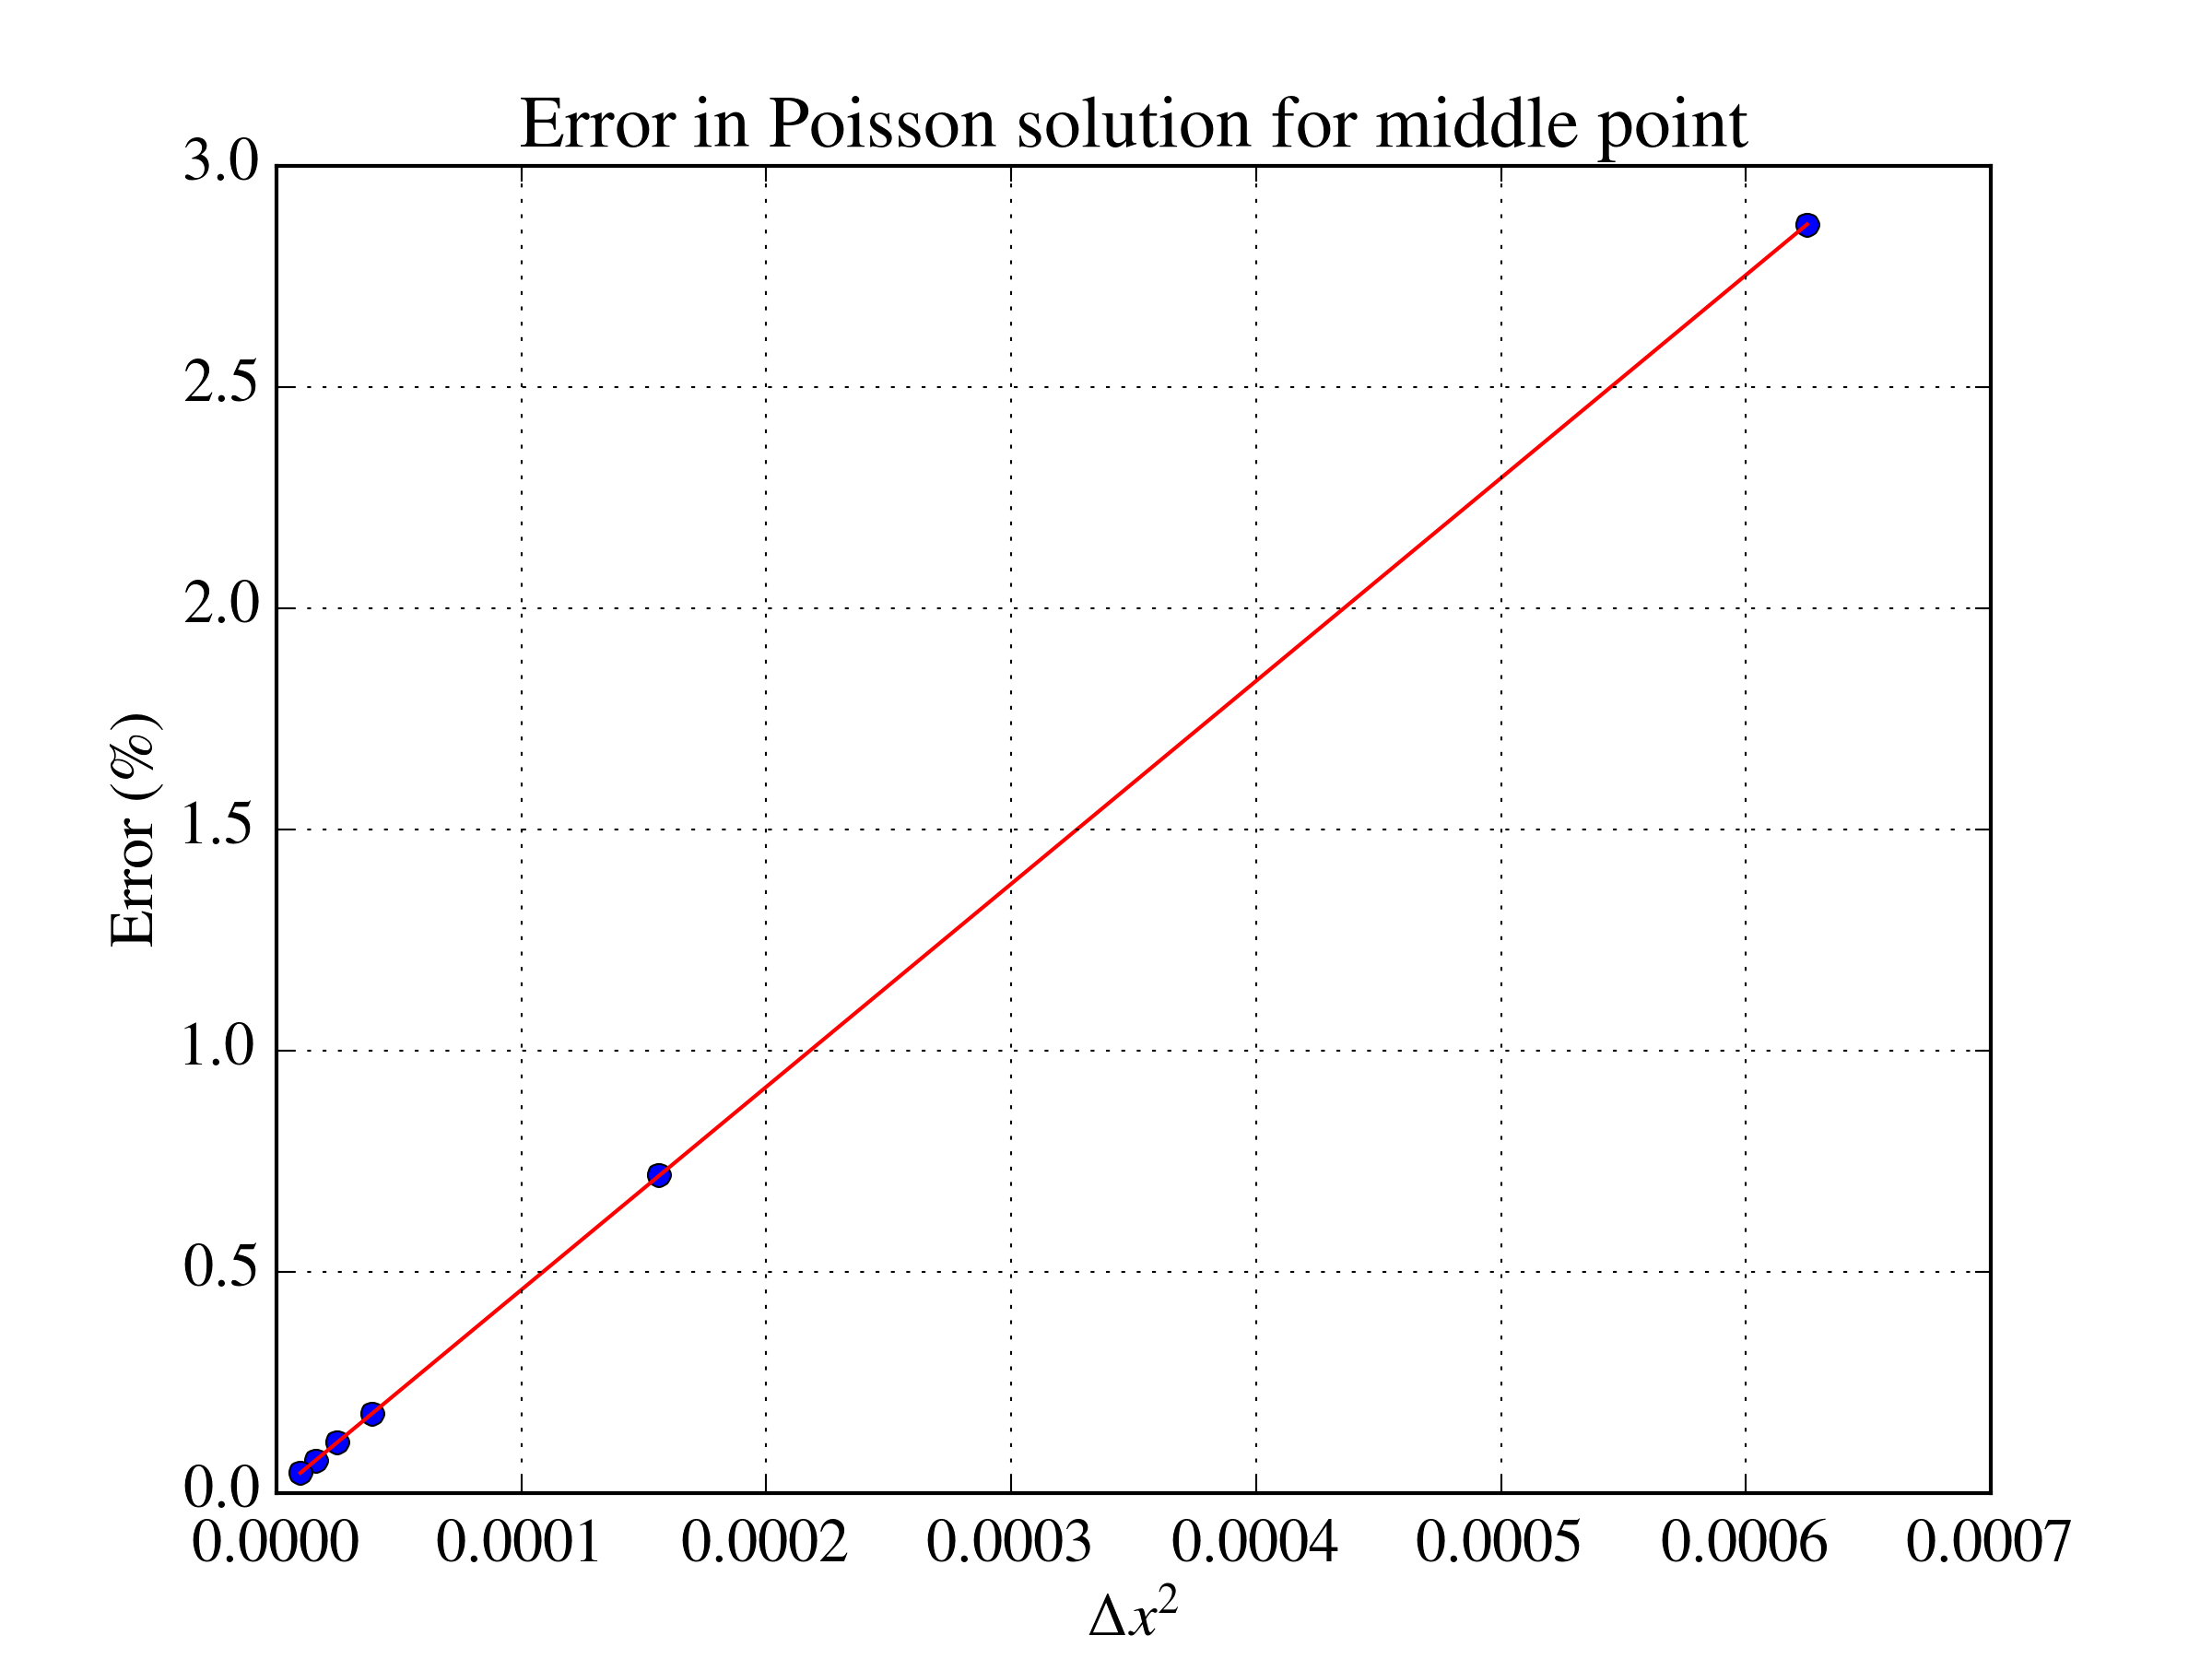
\includegraphics[width=\linewidth]{figures/validatePoissonP2}
\caption{Error evolving according to grid size. Grid sizes with higher number of points are closer to left-bottom corner. Error decays quadratically. Comparison with analytical solution. Grid sizes from $40\times 40$ to $320\times 320$. \label{errorPoissonTest}}
\end{figure}

\subsection{Validation of the Navier-Stokes routine}

Validation for the hydrodynamics is presented on Figure \ref{hydrodynamicsTest}. Reynolds is chosen to be 40. The error will be compared against the solution of grid size $200\times 200$, as access to the analytical solution is not possible. The important point to evaluate is that the error decays quadratically, what can be assessed from the image for simplicity. Vorticity was used instead of velocity because it is a scalar that accounts for both velocity terms. Note that the error corresponds to the base case of $200\times 200$.

\begin{figure}[!t]
\centering
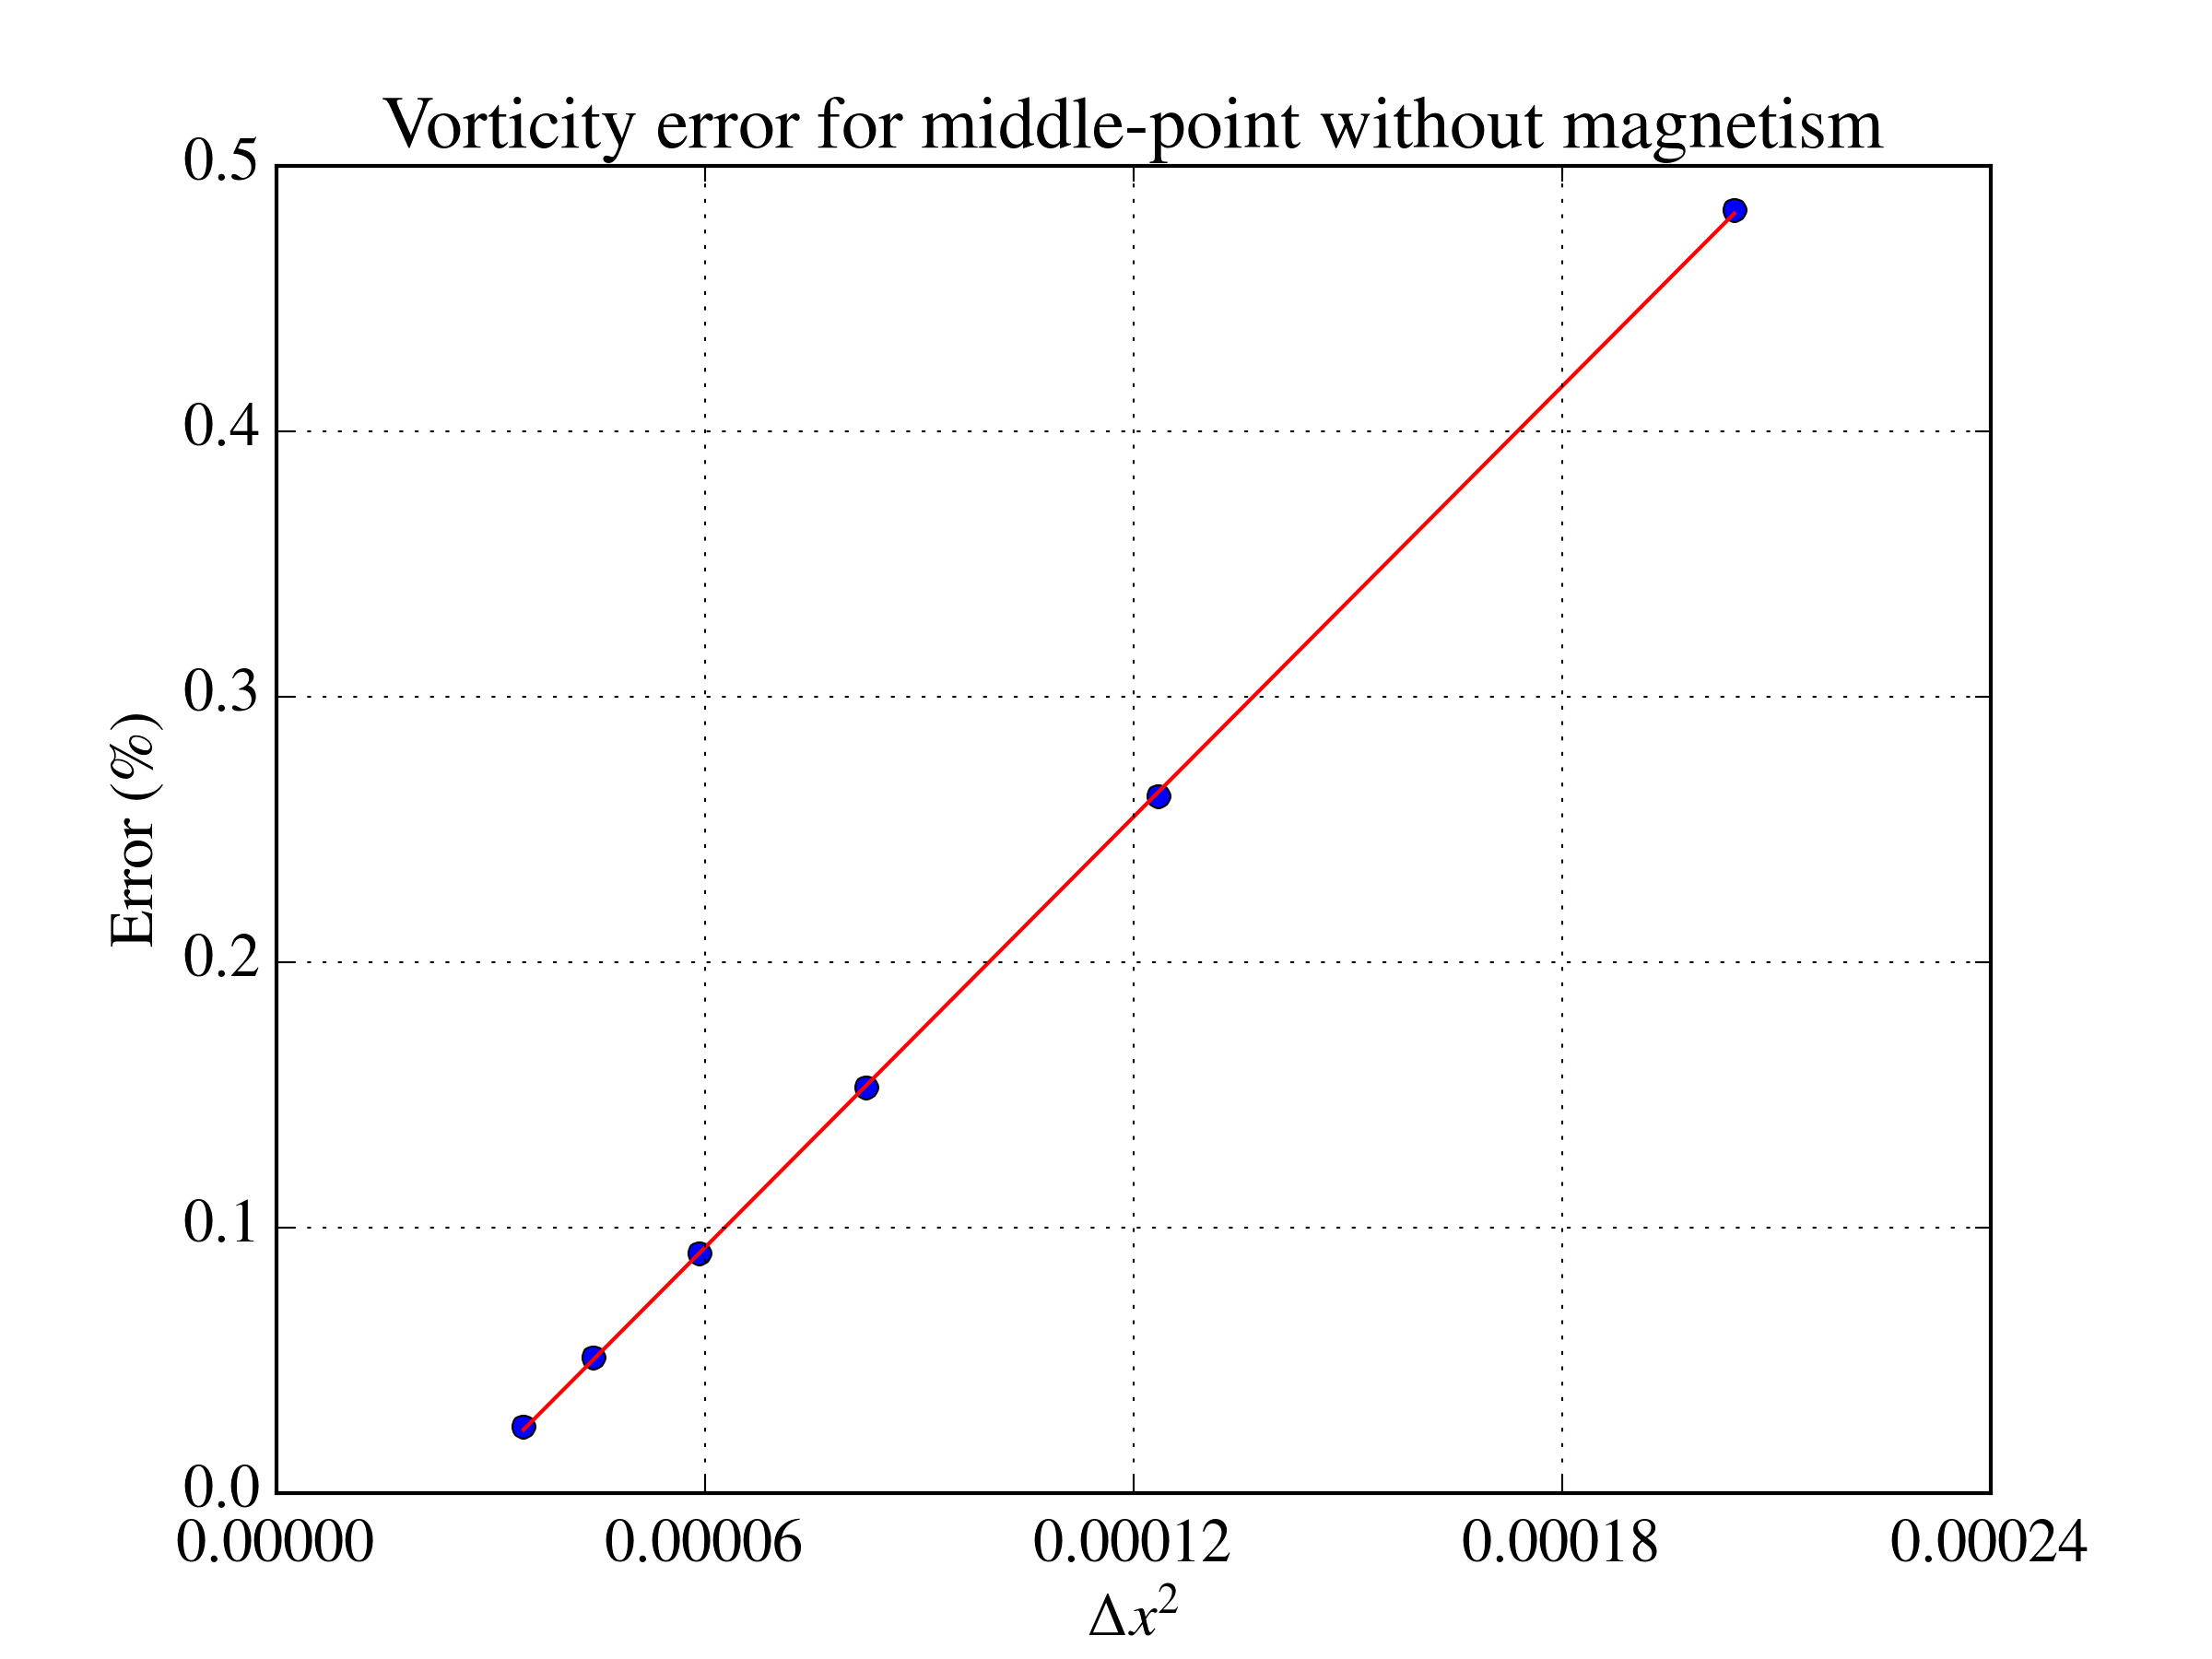
\includegraphics[width=\linewidth]{figures/validateHydrodynamicsRe40}
\caption{Error evolving according to grid size. Higher grid sizes are closer to left-bottom corner. Error decays quadratically. Comparison with solution of $200\times 200$ grid. Grid sizes from $70\times 70$ to $170\times 170$. \label{hydrodynamicsTest}}
\end{figure}

A similar test was used when magnetism is present. This case has a force $\mathbf{f}$ that differs from zero. Magnetic parameters chosen are $\chi=0.5$, $\mathrm{C}_\mathrm{pm}=0.8$, $\gamma=3$ and a center for the magnetic field located close the left-bottom corner. The applied magnetic field is that depicted in Figure \ref{magneticField}. The magnetic field is $\mathbf{H}=(H_x,H_y)$, whose components are given by: \begin{eqnarray}
H_x(x,y) & = & \frac{\gamma}{2\pi} \frac{y - b}{(x-a)^2+(y-b)^2},\label{Hx}\\
H_y(x,y) & = & -\frac{\gamma}{2\pi} \frac{x - a}{(x-a)^2+(y-b)^2},\label{Hy}
\end{eqnarray} where $(a,b)$ is the point where the magnetic source is placed and $\gamma$ is the magnetic field strength at this point \cite{Tzirtzilakis2013}. The terms just presented are already dimensionless. The error evolution for the case presented is on Figure \ref{magneticTest}, where the values were compared in steady-state.


\begin{figure}[!t]
\centering
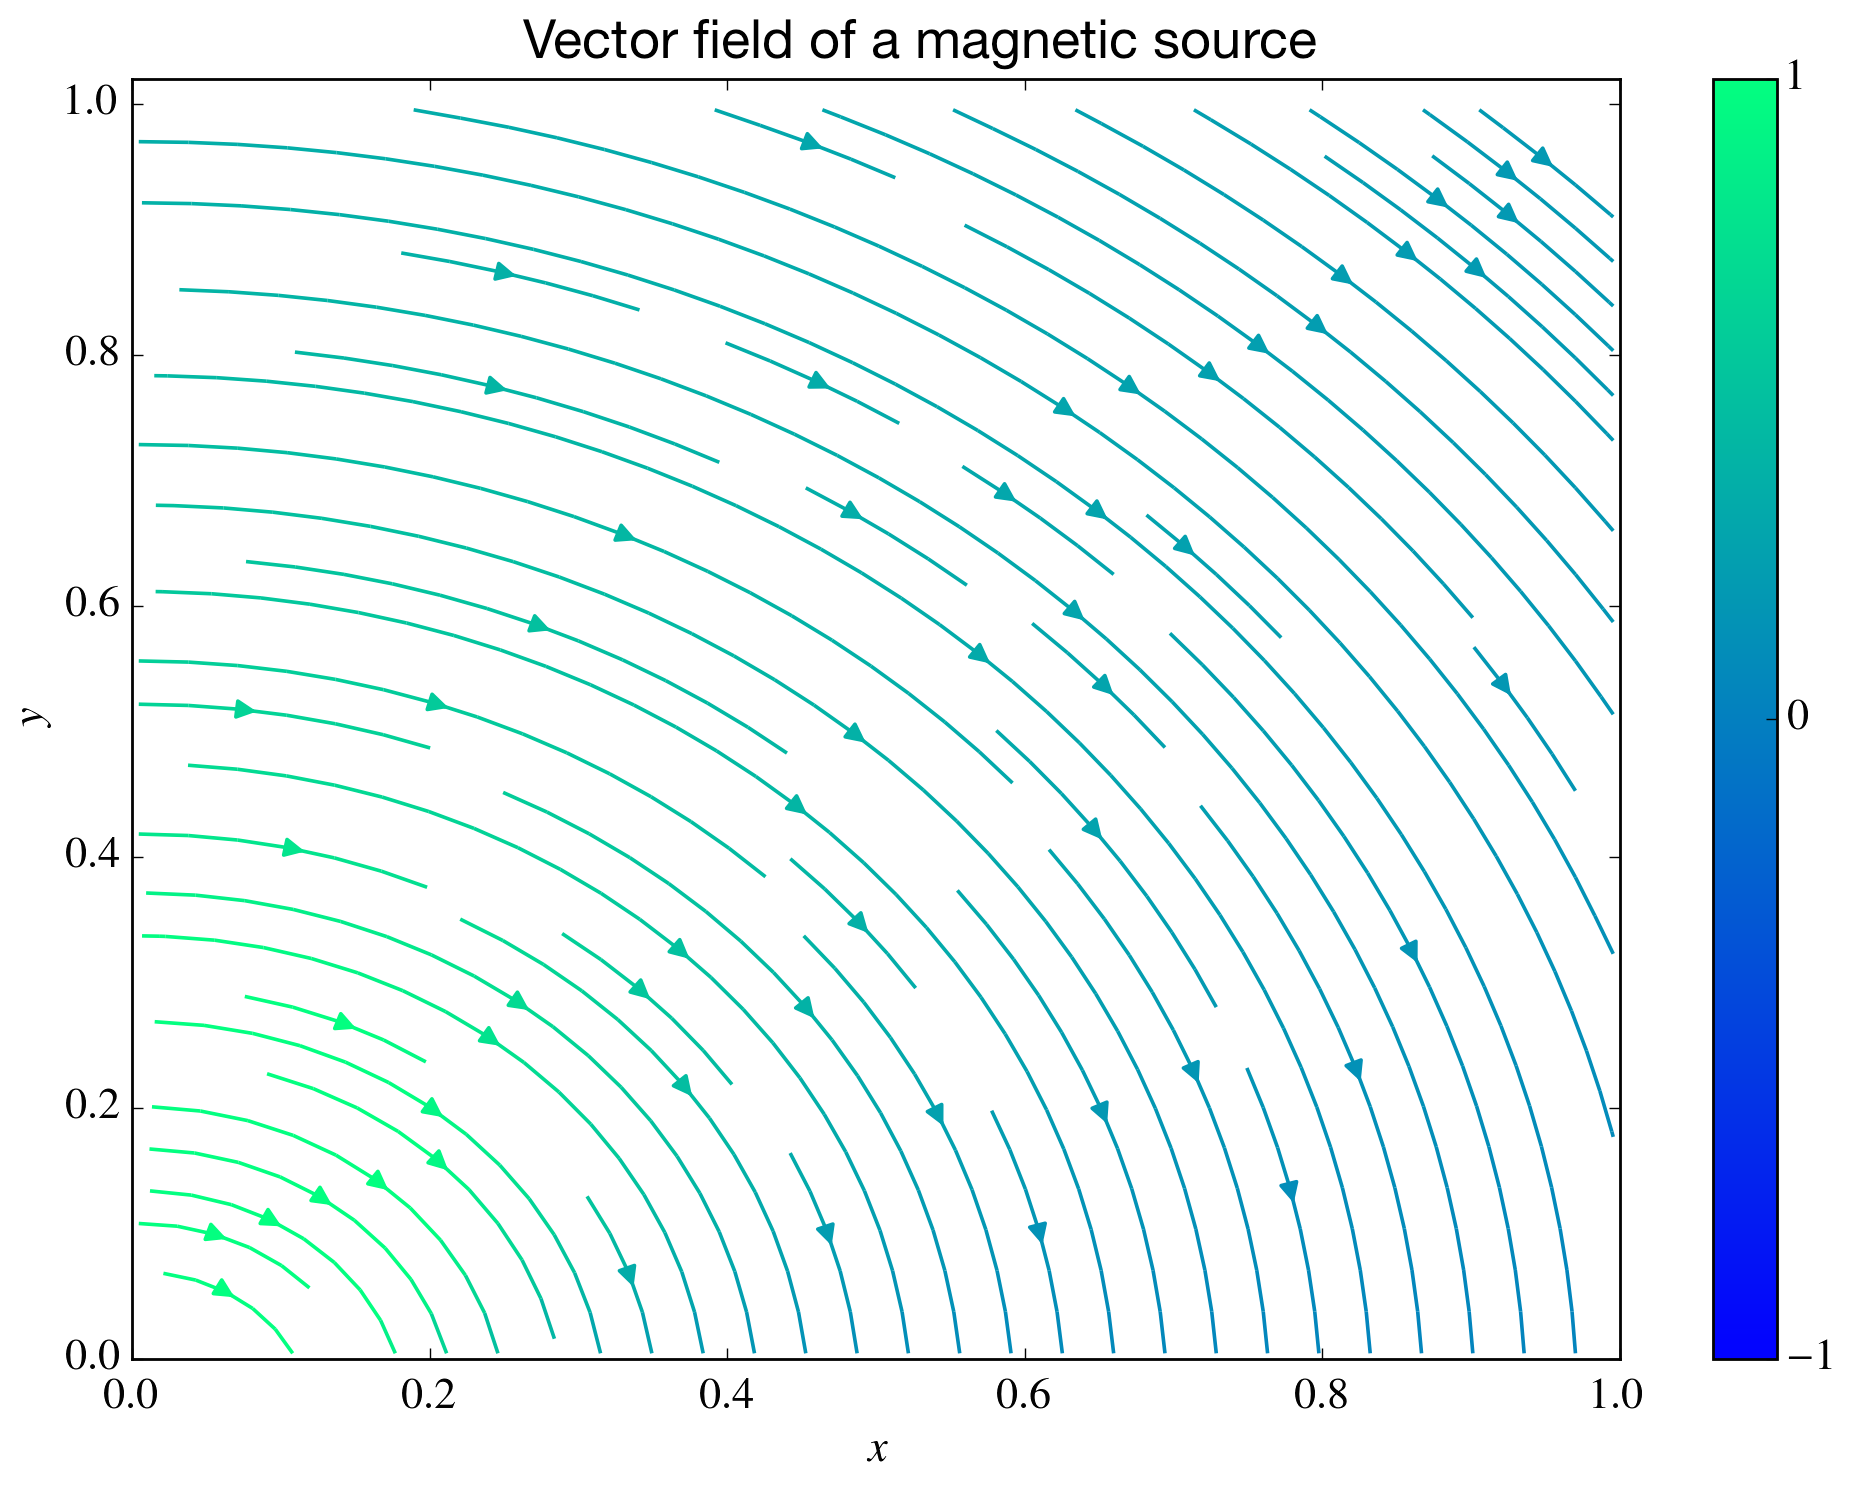
\includegraphics[width=\linewidth]{figures/vectorFieldH}
\caption{Applied magnetic field. All tests were made with this specific magnetic field. $\gamma$ values may change the actual intensity of field, but the streamlines are similar.\label{magneticField}}
\end{figure}


\begin{figure}[!t]
\centering
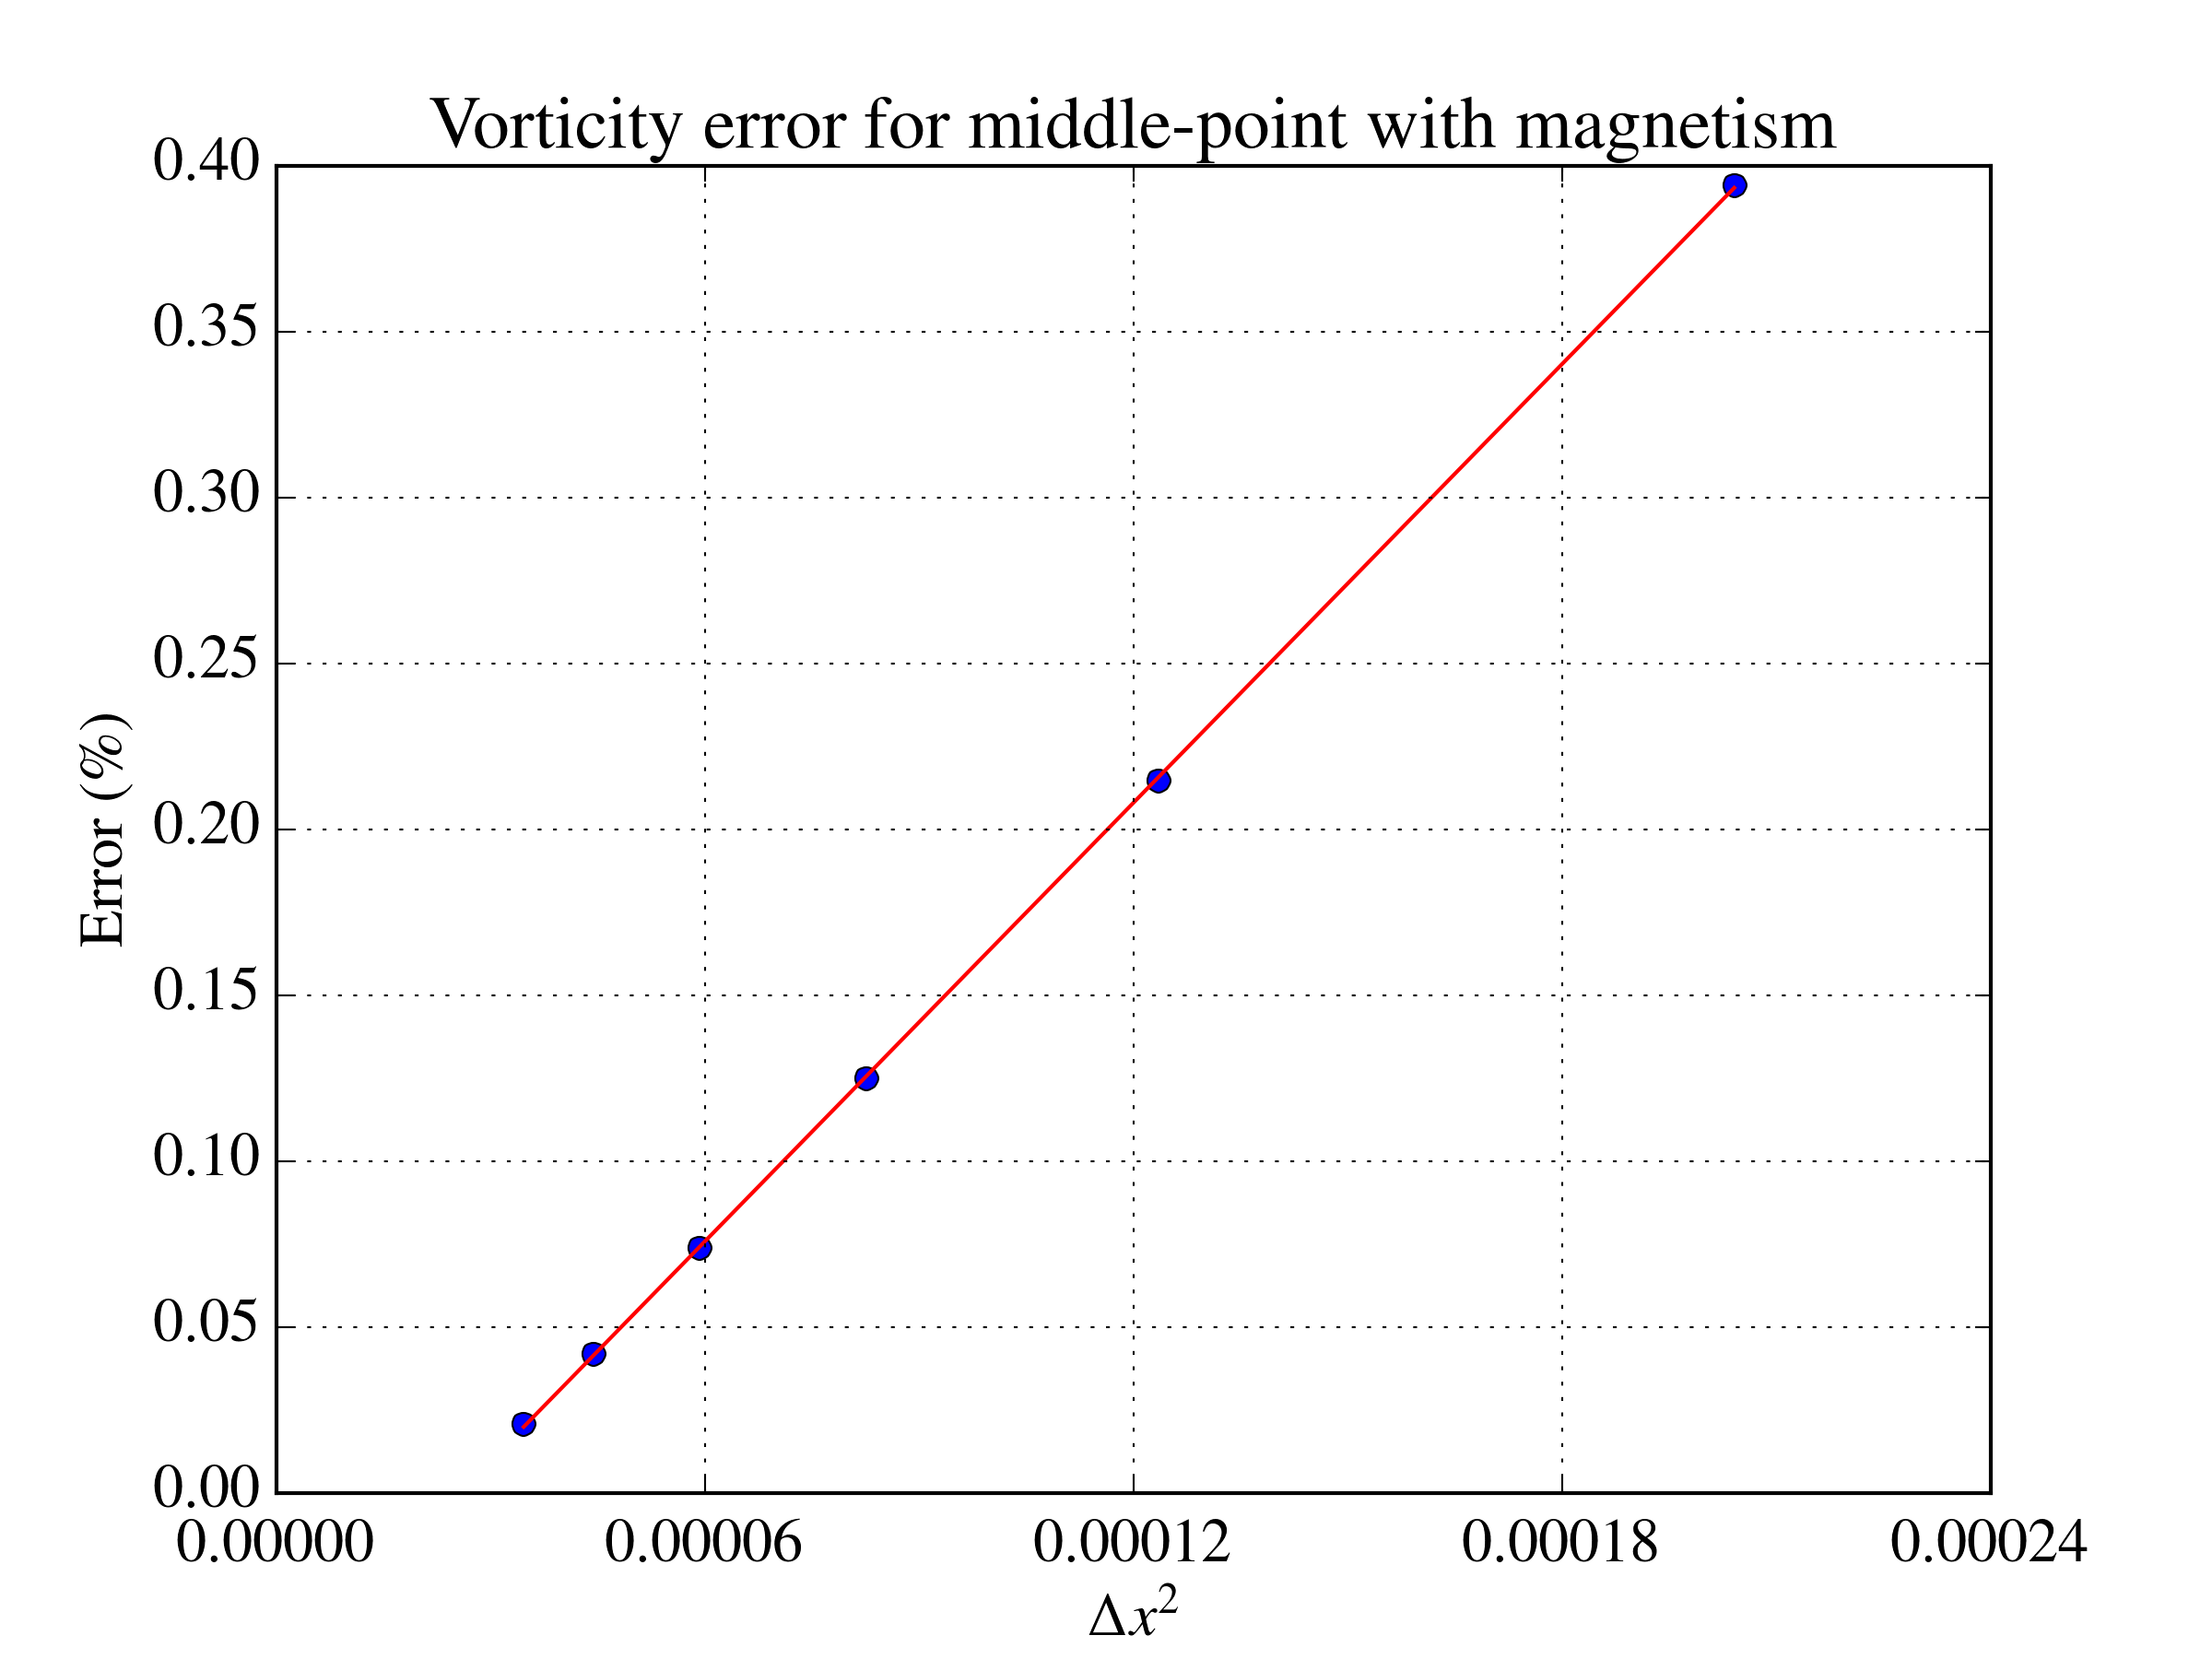
\includegraphics[width=\linewidth]{figures/validateMagnetismRe40}
\caption{Error evolving according to grid size. Higher grid sizes are closer to left-bottom corner. Error decays quadratically. Comparison with solution of $200\times 200$ grid. Grid sizes from $70\times 70$ to $170\times 170$. \label{magneticTest}}
\end{figure}



\subsection{Preliminary studies of flow patterns}
We have performed some tests to assess the influence of the dimensionless parameters $\mathit{Re}$ and $\mathrm{C}_\mathrm{pm}$ on the steady-state regimes that were obtained.  Some Reynolds numbers were chosen and then several tests were executed for some fixed magnetic parameters. The magnetic parameters are $\chi=0.5$, $\mathrm{C}_\mathrm{pm}=0.8$ and $\gamma=3.5$. Reynolds numbers presented here are 1, 50 and 100. Figures \ref{Re001nVectorField} to \ref{Re100wPressure} present streamlines for the velocity and contour lines for the pressure. Images with magnetic parameters set to 0 are the ones without magnetization. All results are in steady state. We have also coded a routine to calculate the angle between $\mathbf{M}$ and $\mathbf{H}$ for every point in those simulations but, for the case presented here, this is not relevant, as $\mathbf{M}=\chi\mathbf{H}$ is one consideration for the magnetization in the current work (superparamagnetic regime).

\begin{figure}[!t]
\centering
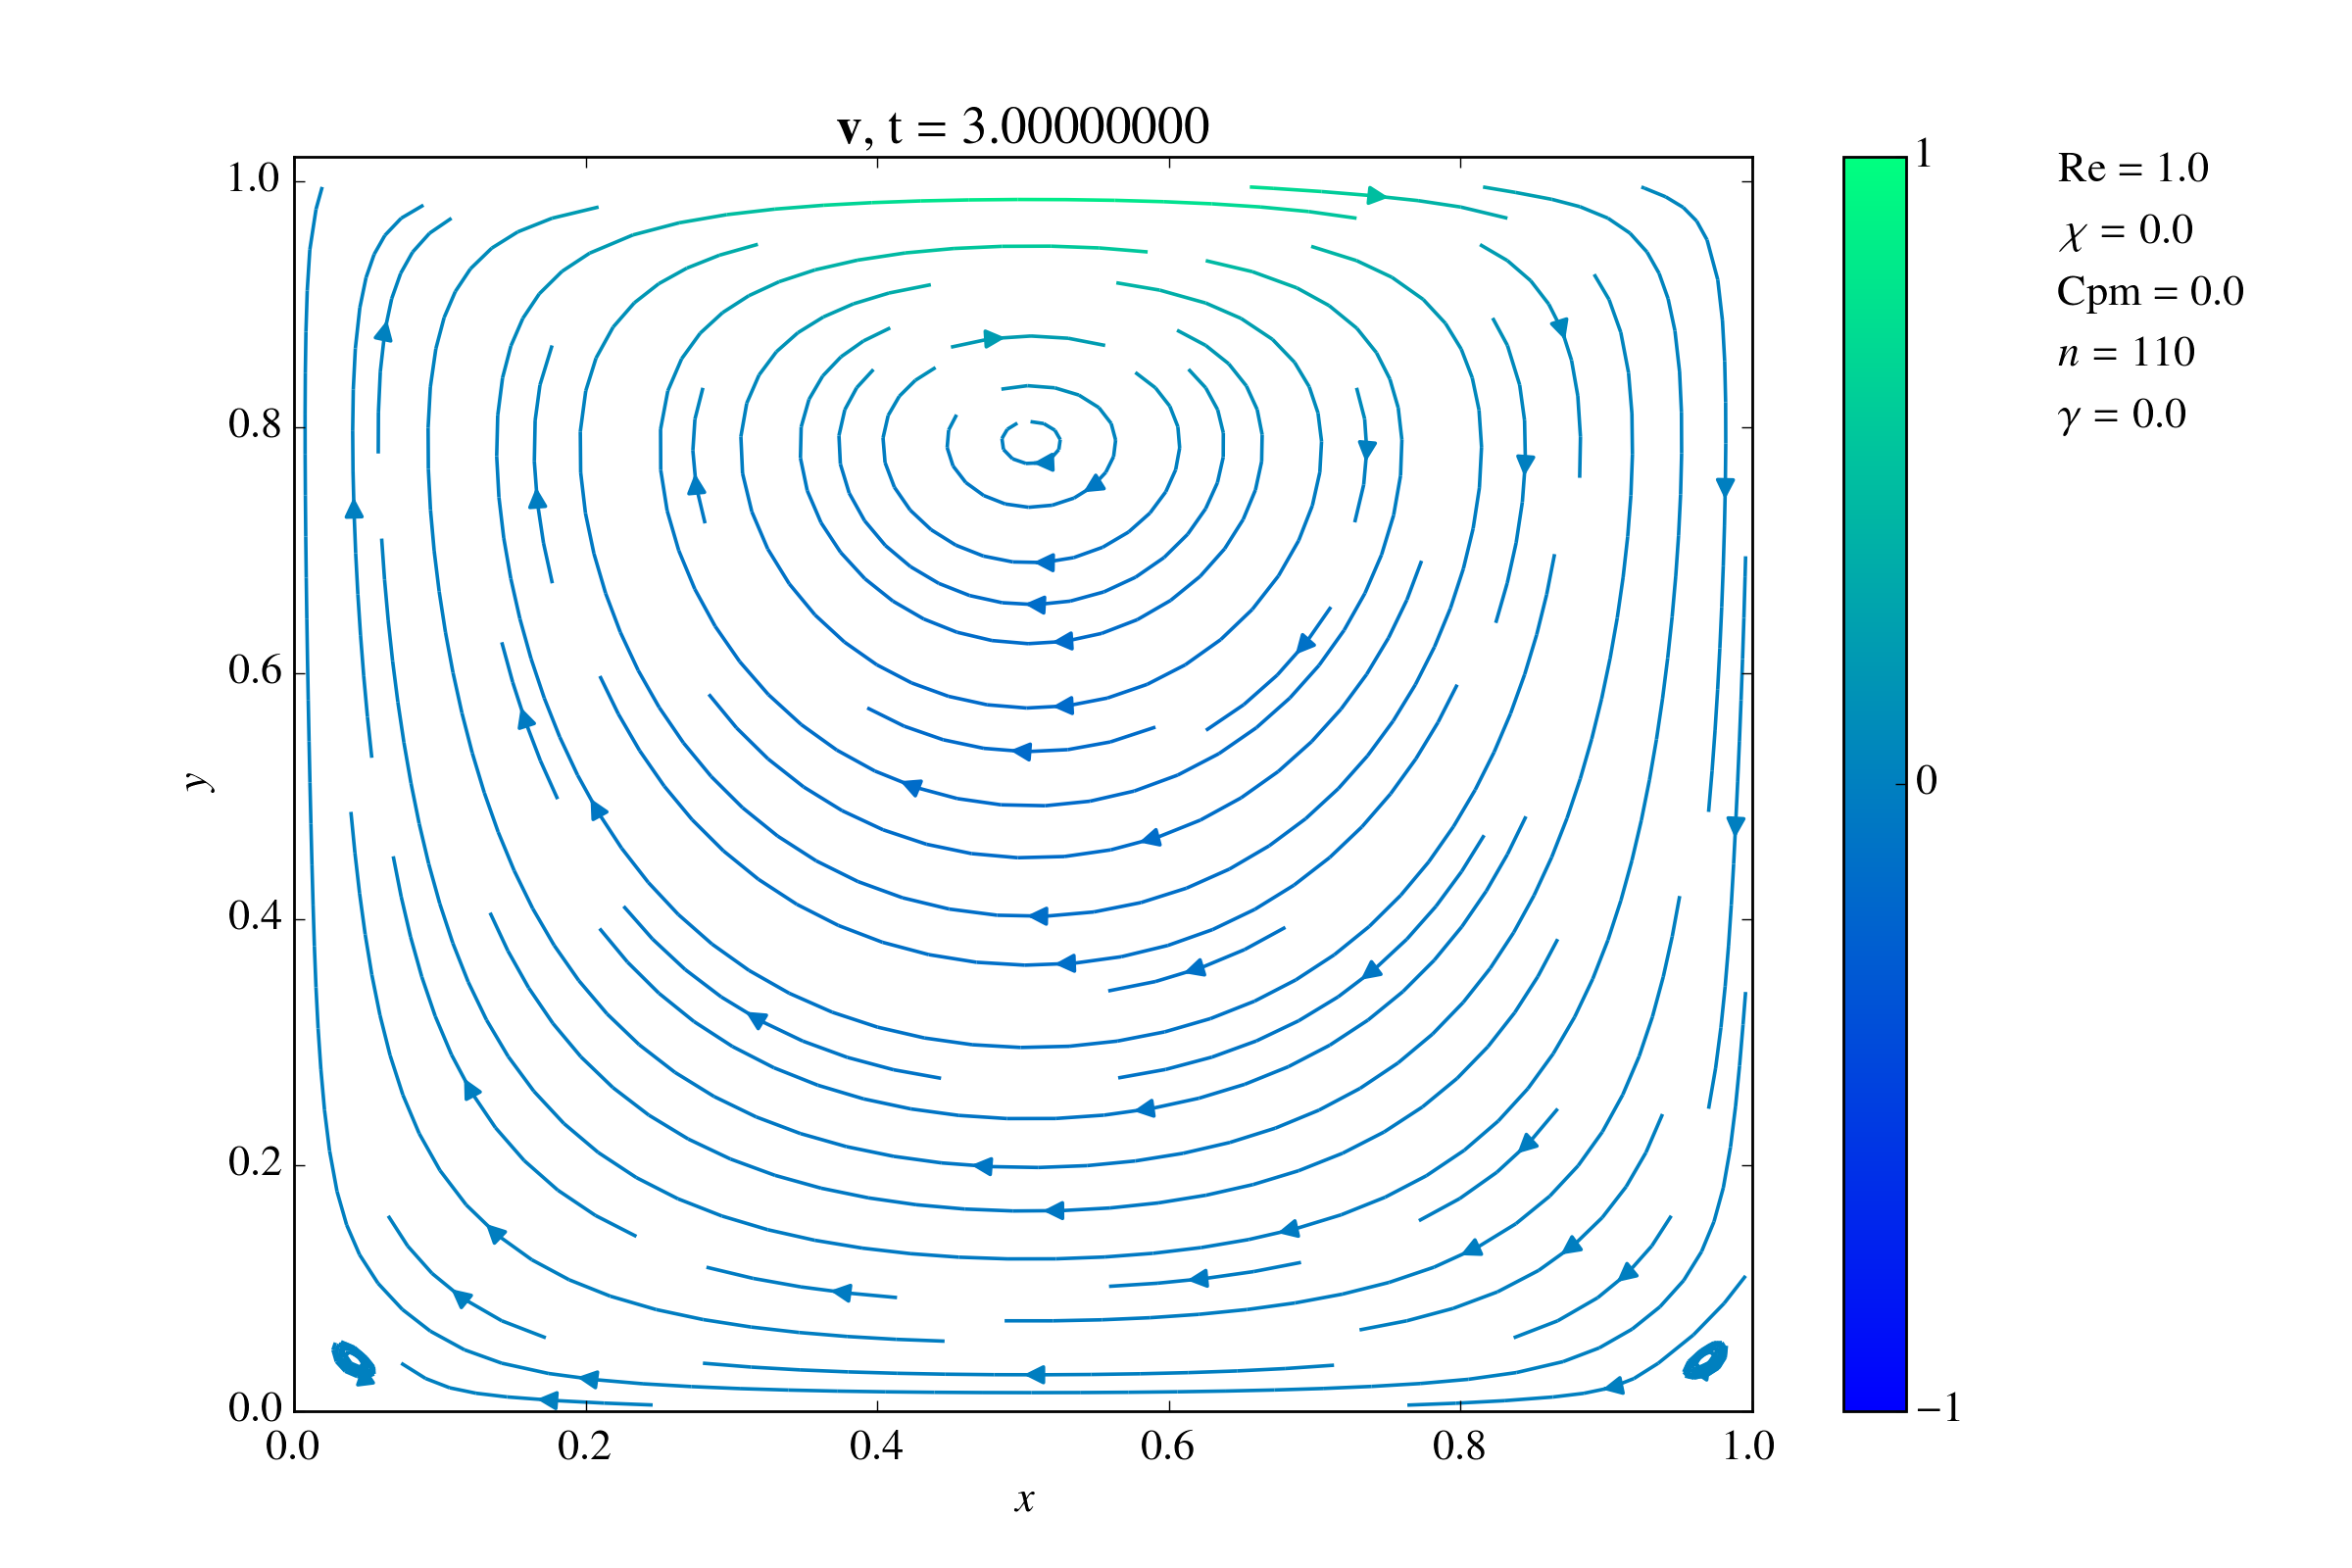
\includegraphics[width=\linewidth]{figures/Re001/n/vectorField}
\caption{Steady state solution without magnetic field, $\mathit{Re}=1$. No extra vortices appear.\label{Re001nVectorField}}
\end{figure}

\begin{figure}[!t]
\centering
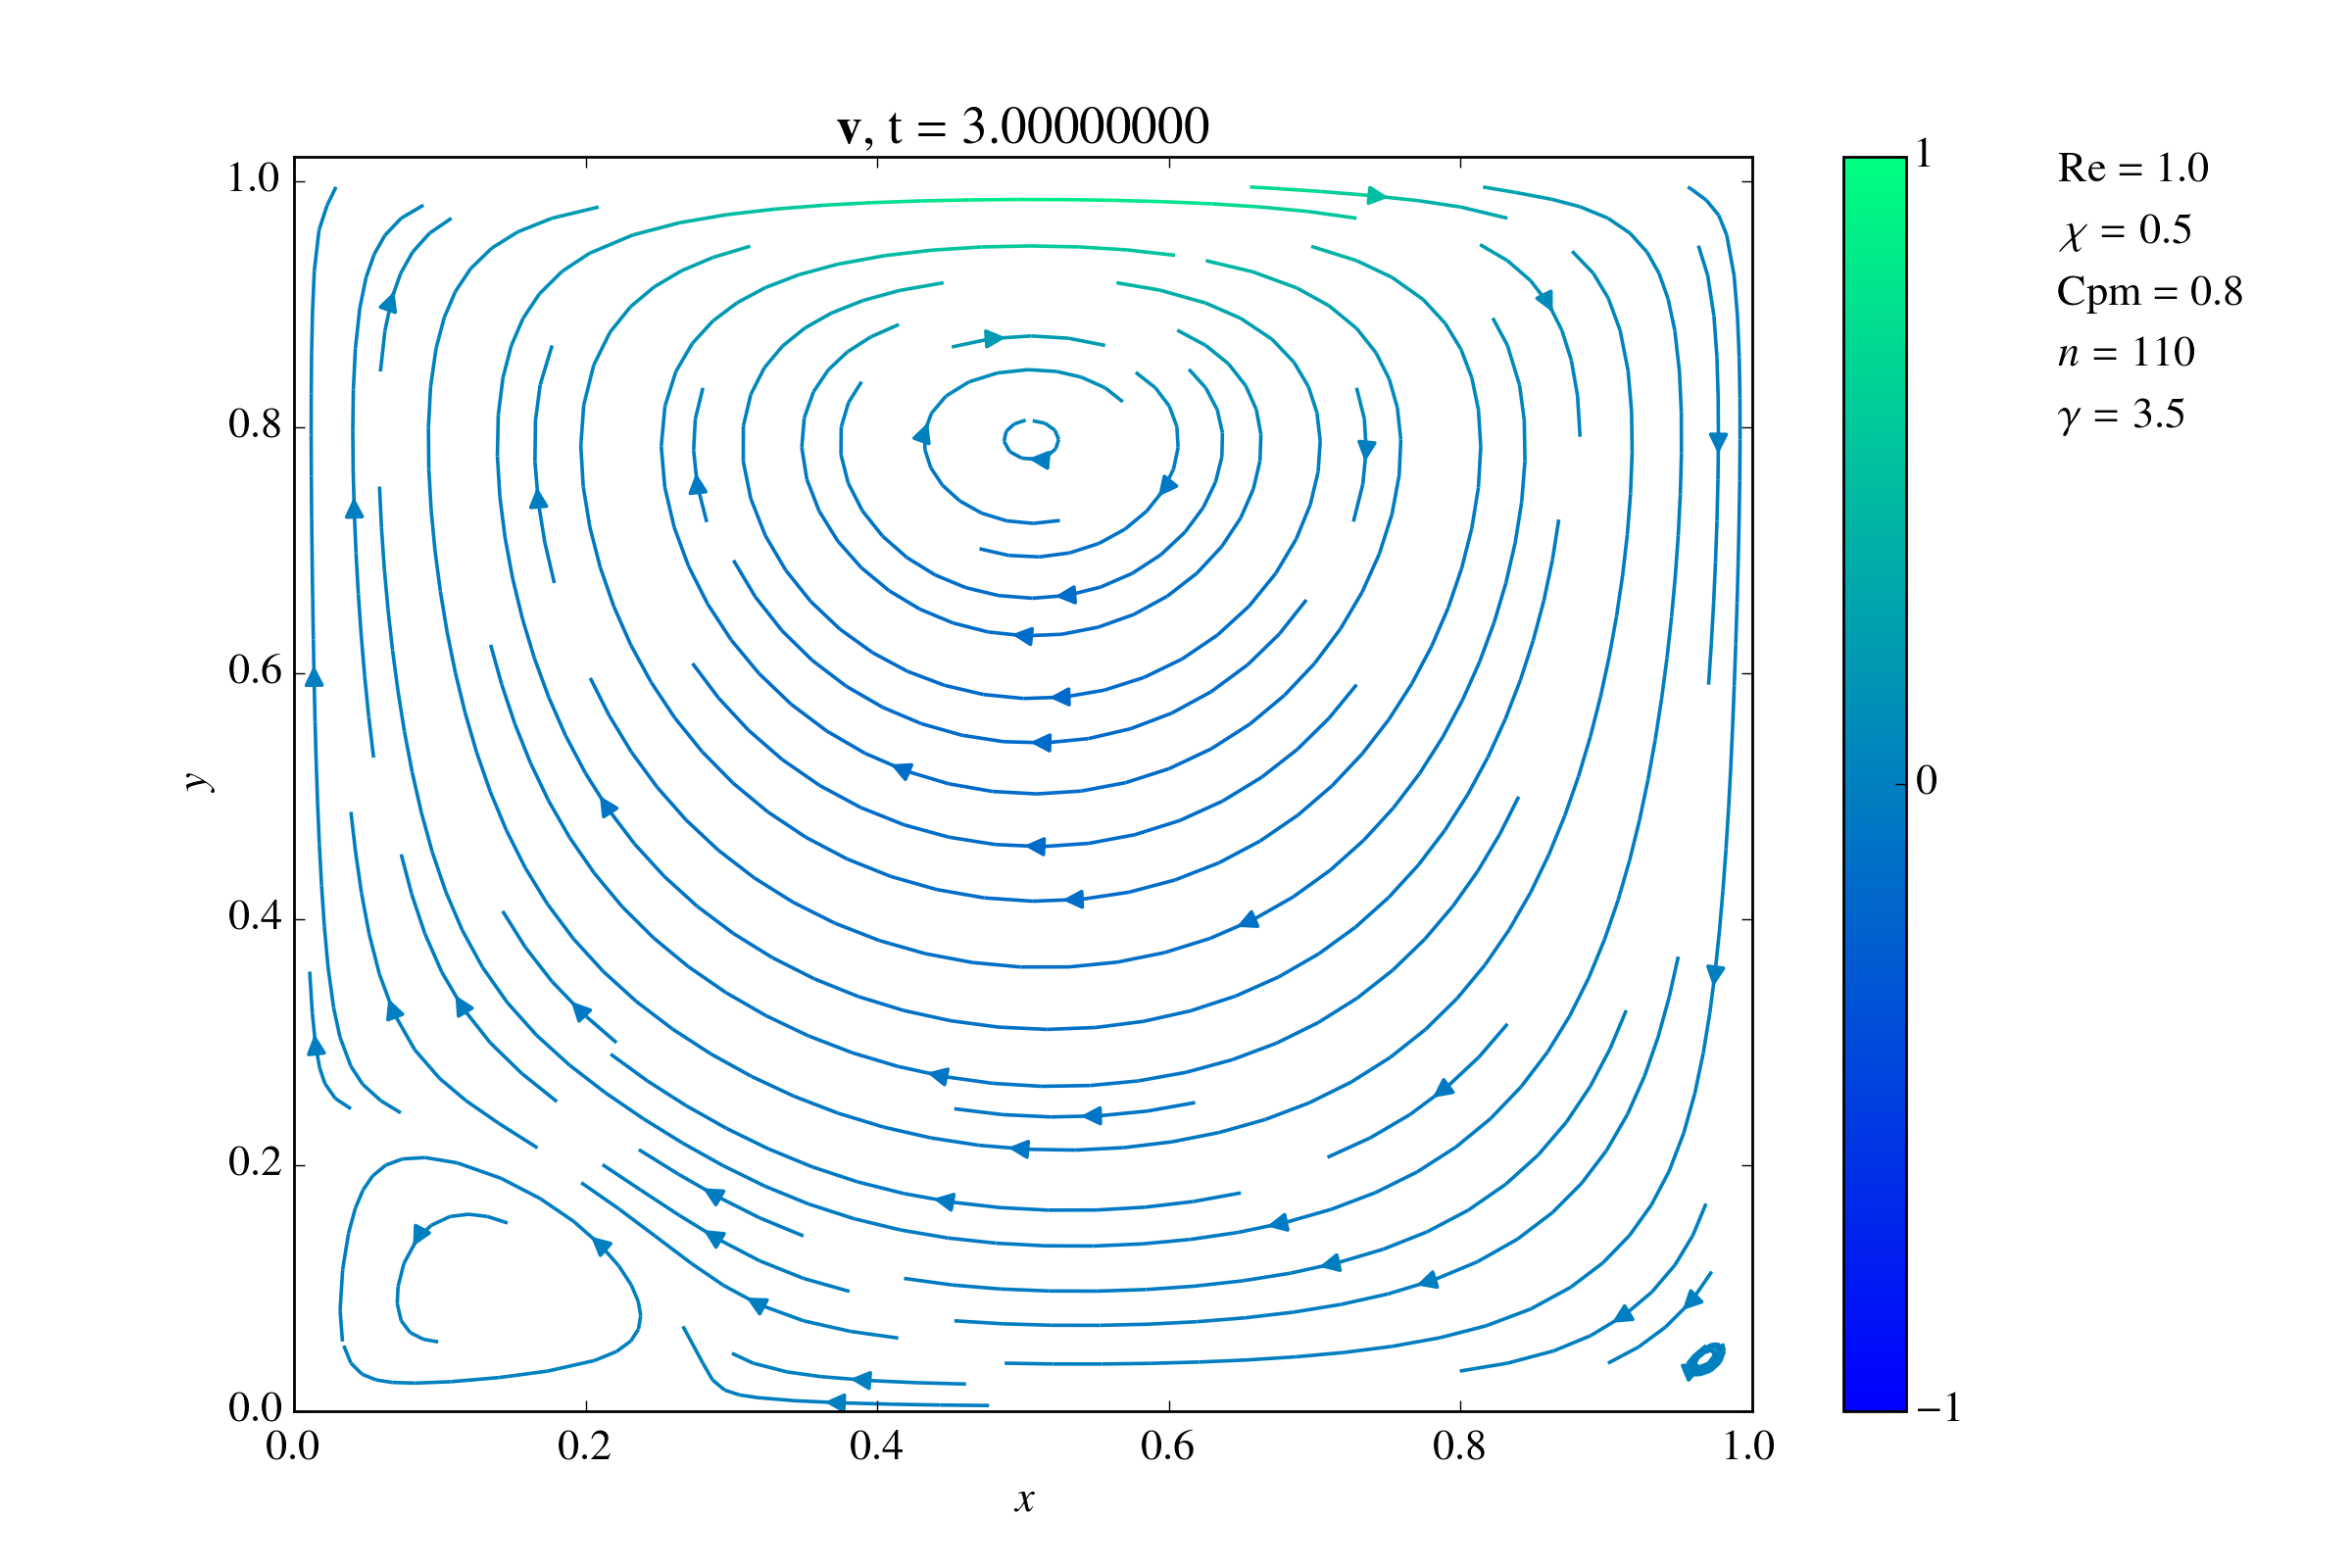
\includegraphics[width=\linewidth]{figures/Re001/w/vectorField}
\caption{Steady state solution with magnetic field, $\mathit{Re}=1$. A new vortex starts to appear. \label{Re001wVectorField}}
\end{figure}

\begin{figure}[!t]
\centering
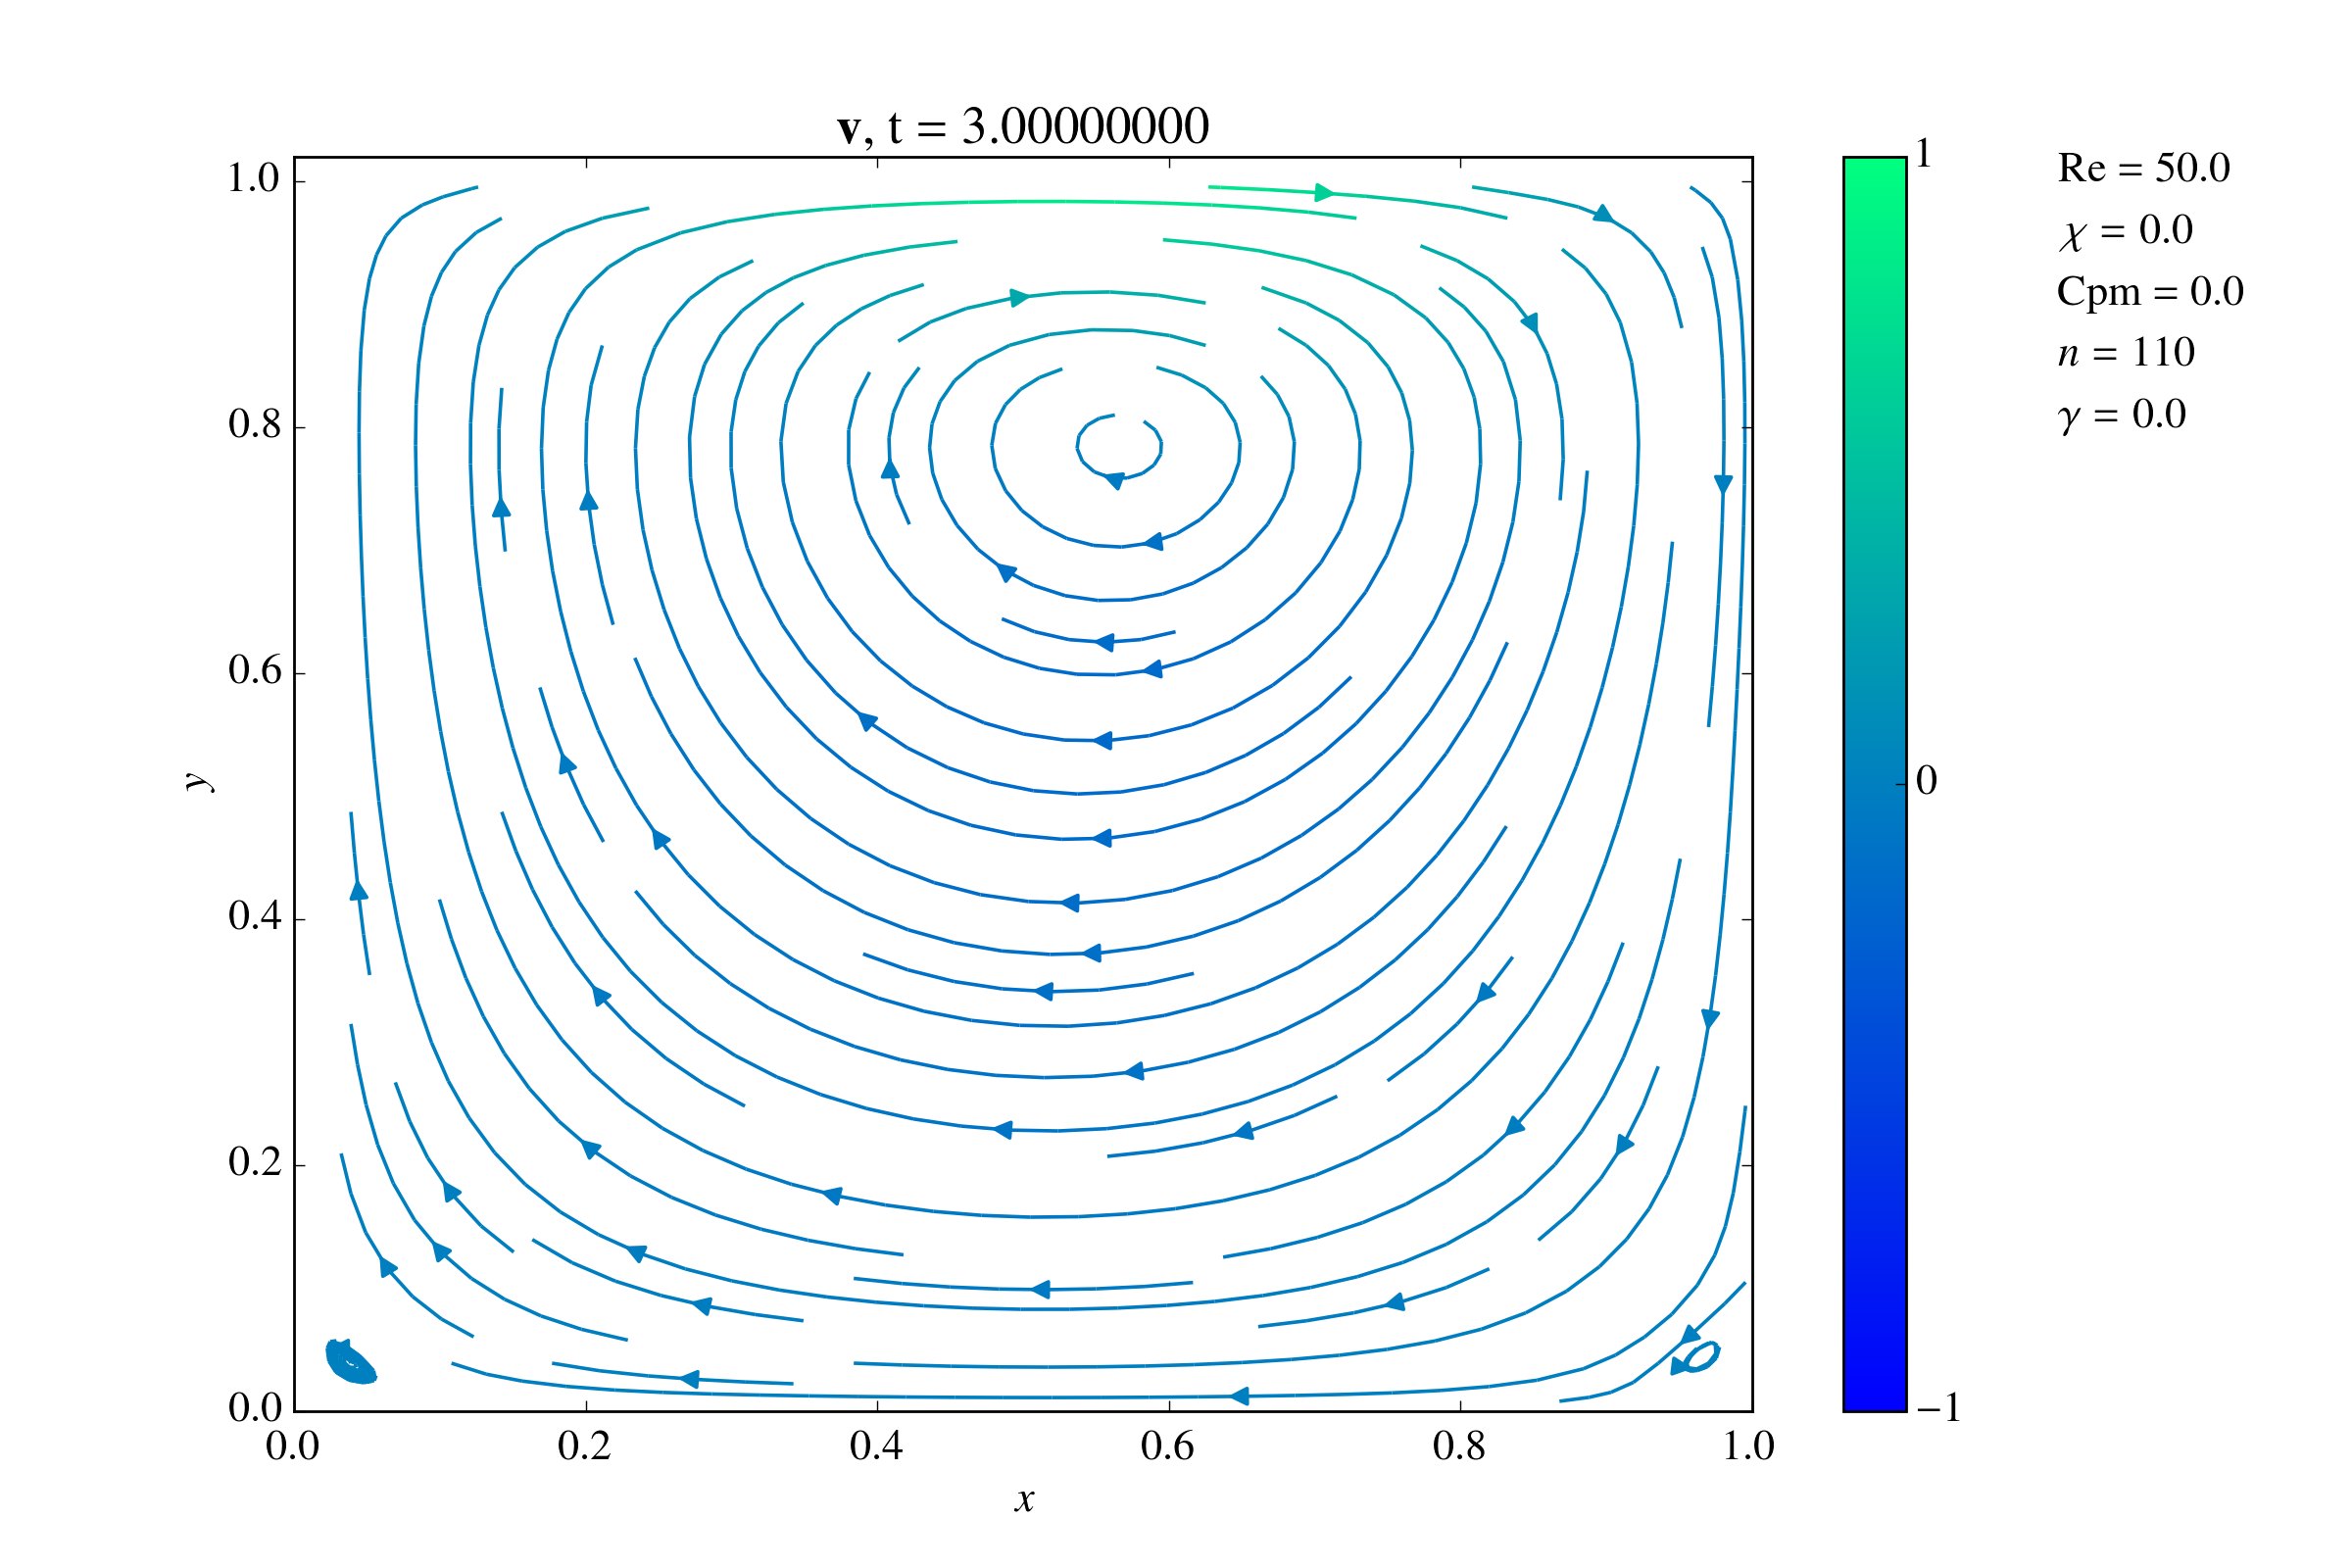
\includegraphics[width=\linewidth]{figures/Re050/n/vectorField}
\caption{Steady state solution without magnetic field, $\mathit{Re}=50$. No extra vortices appear. \label{Re050nVectorField}}
\end{figure}

\begin{figure}[!t]
\centering
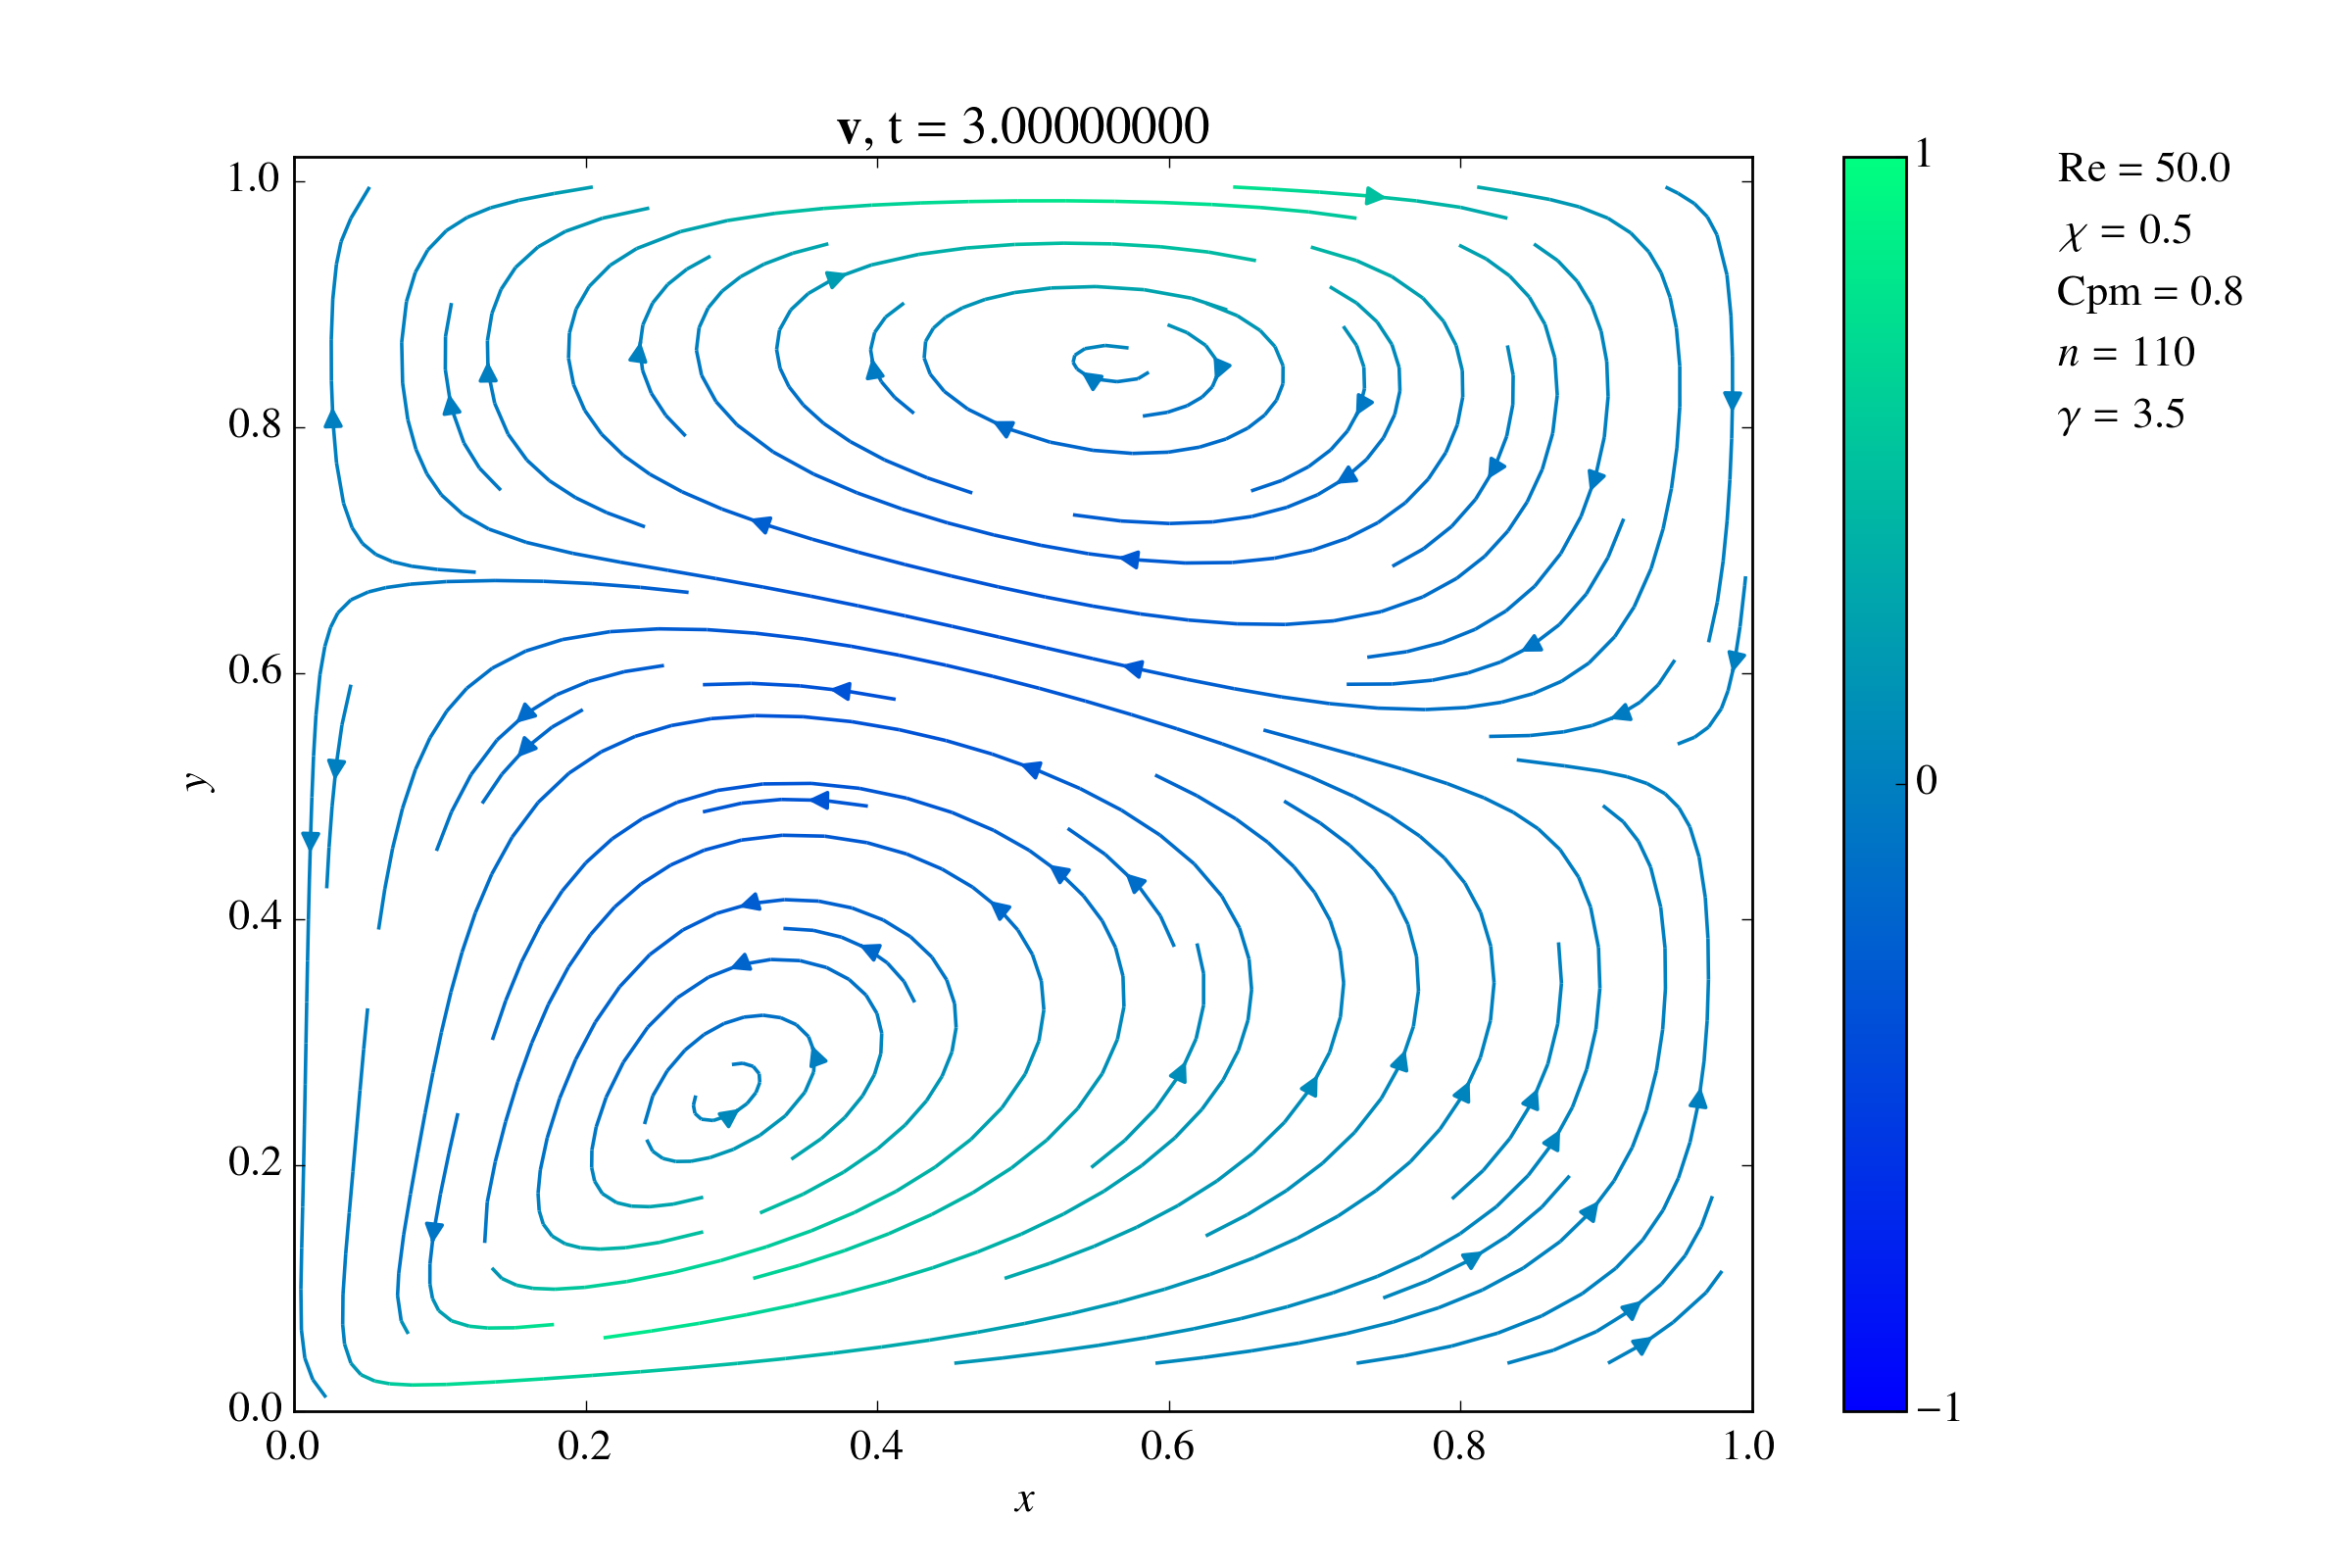
\includegraphics[width=\linewidth]{figures/Re050/w/vectorField}
\caption{Steady state solution with magnetic field, $\mathit{Re}=50$. The new vortex is already bigger than the initial one. \label{Re050wVectorField}}
\end{figure}

\begin{figure}[!t]
\centering
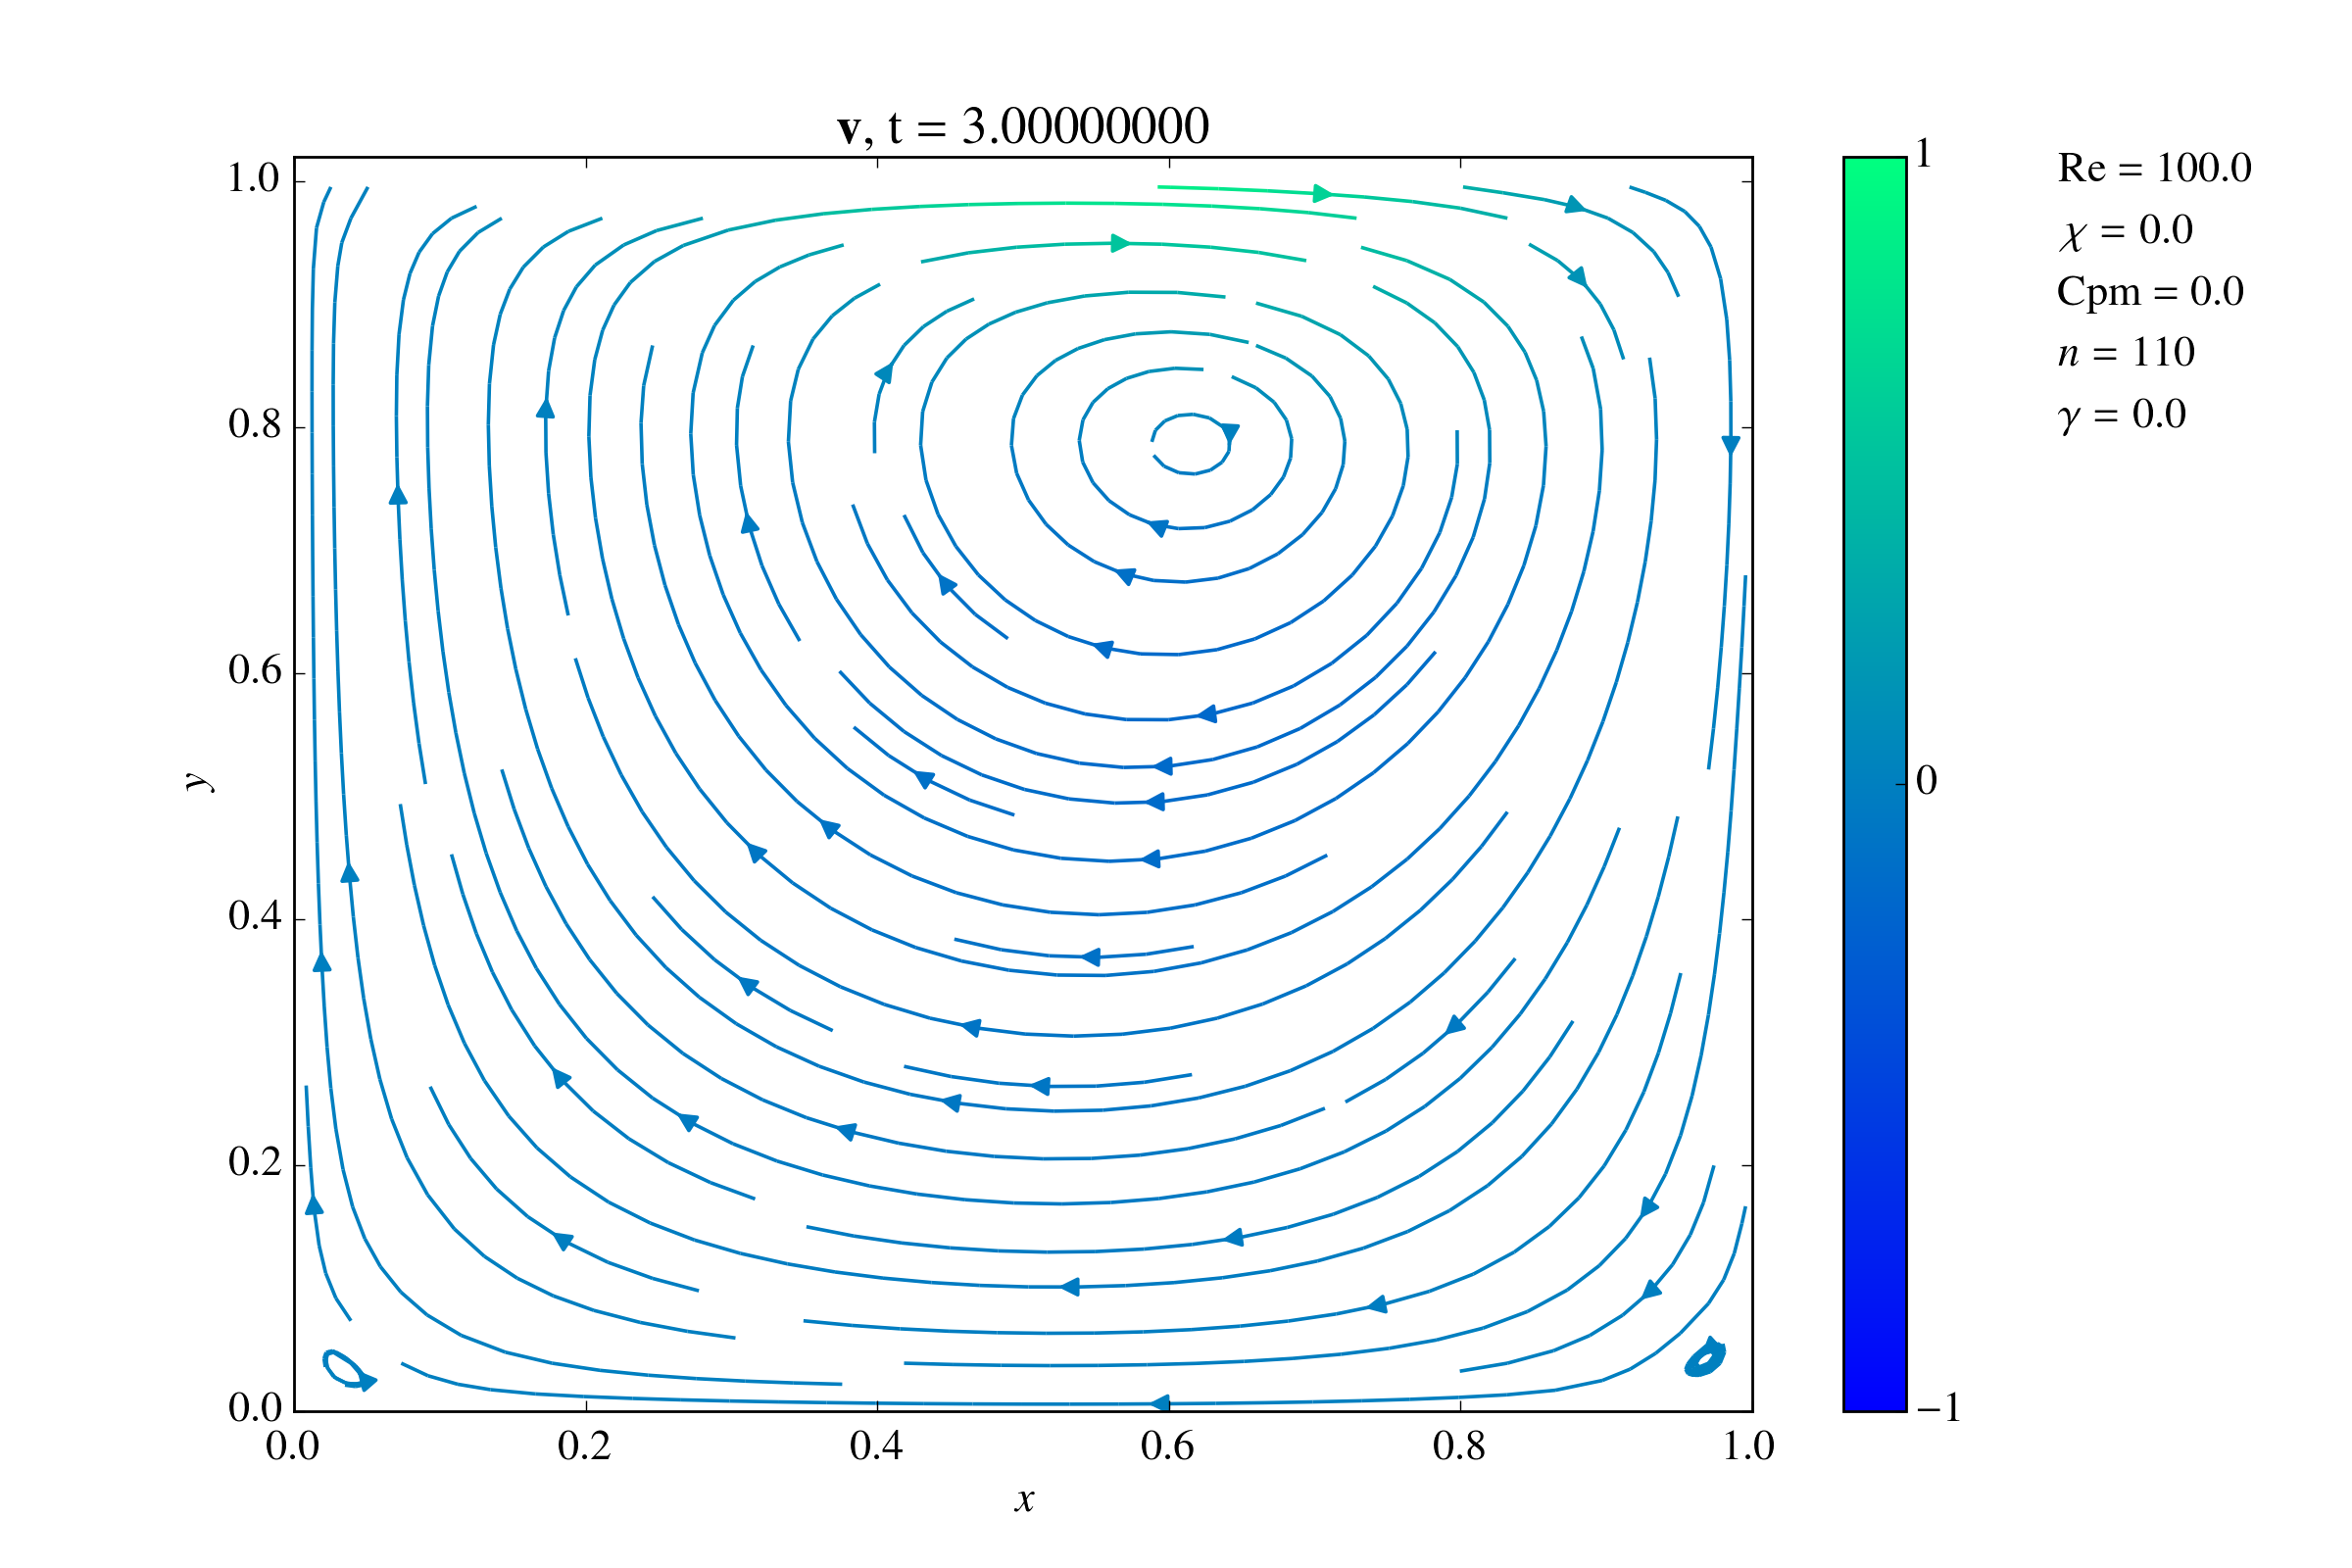
\includegraphics[width=\linewidth]{figures/Re100/n/vectorField}
\caption{Steady state solution without magnetic field, $\mathit{Re}=100$. No extra vortices appear. \label{Re100nVectorField}}
\end{figure}

\begin{figure}[!t]
\centering
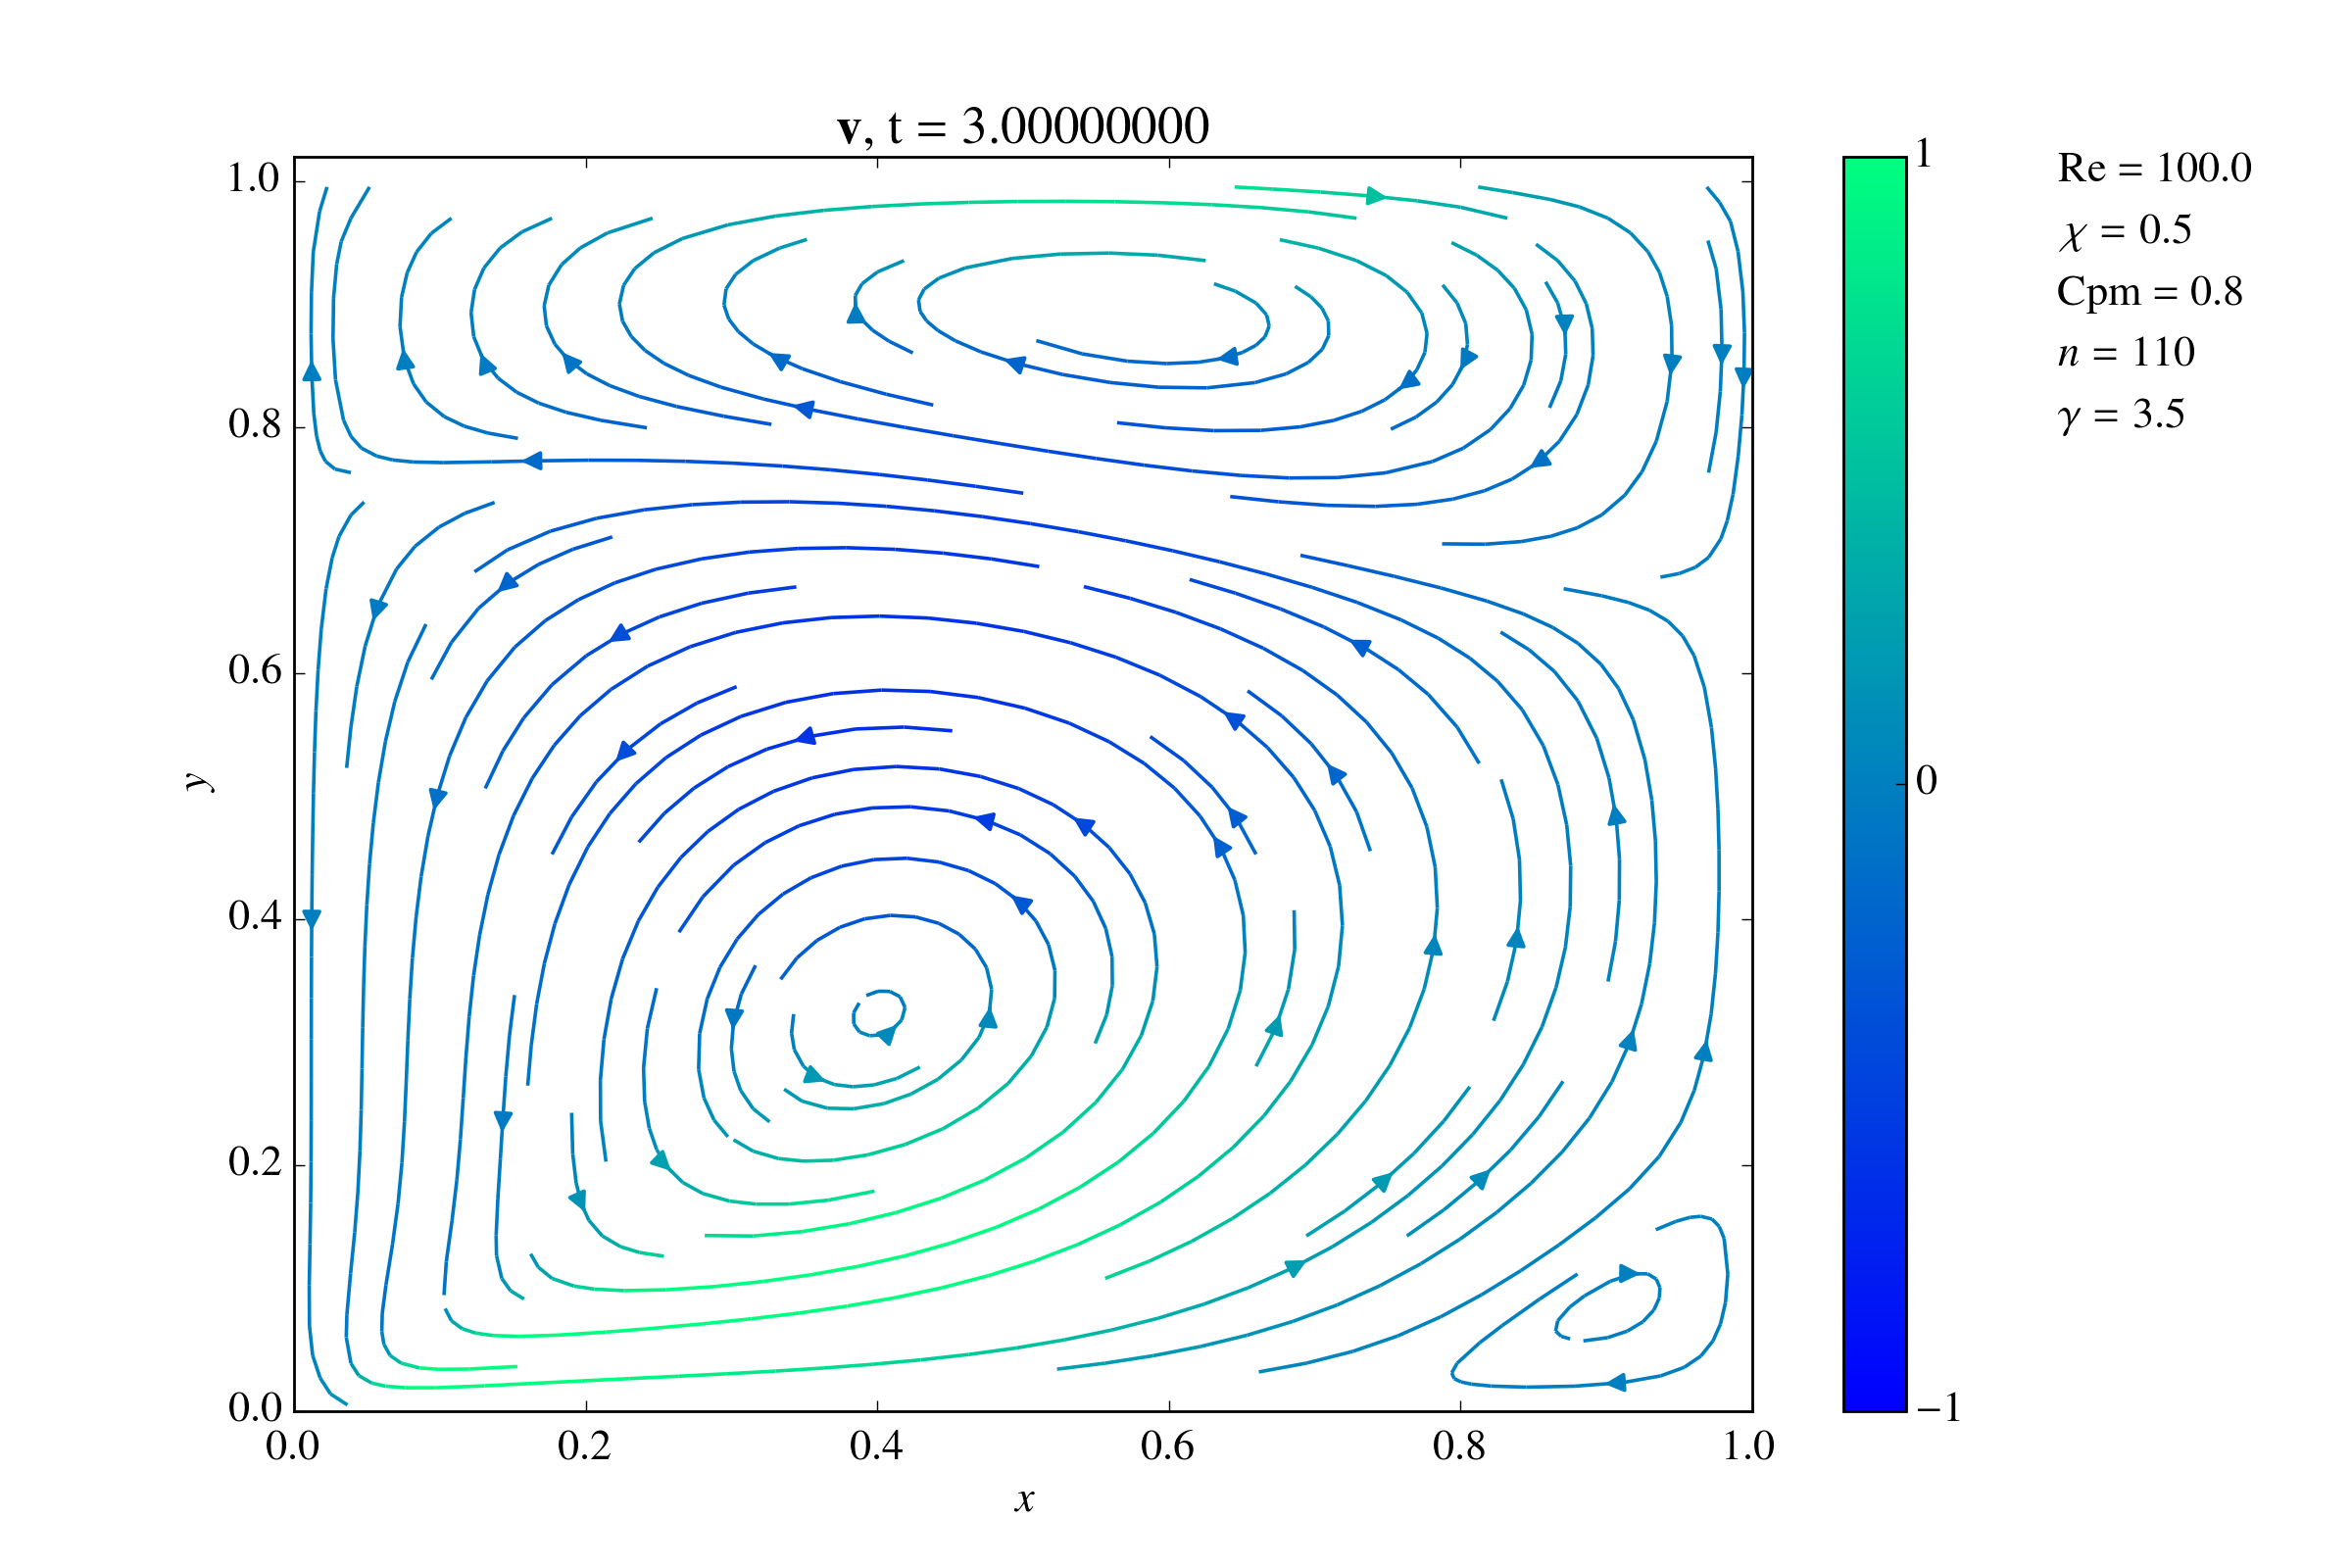
\includegraphics[width=\linewidth]{figures/Re100/w/vectorField}
\caption{Steady state solution with magnetic field, $\mathit{Re}=100$. Vortex increased in comparison with $\mathit{Re} = 50$. \label{Re100wVectorField}}
\end{figure}


\begin{figure}[!t]
\centering
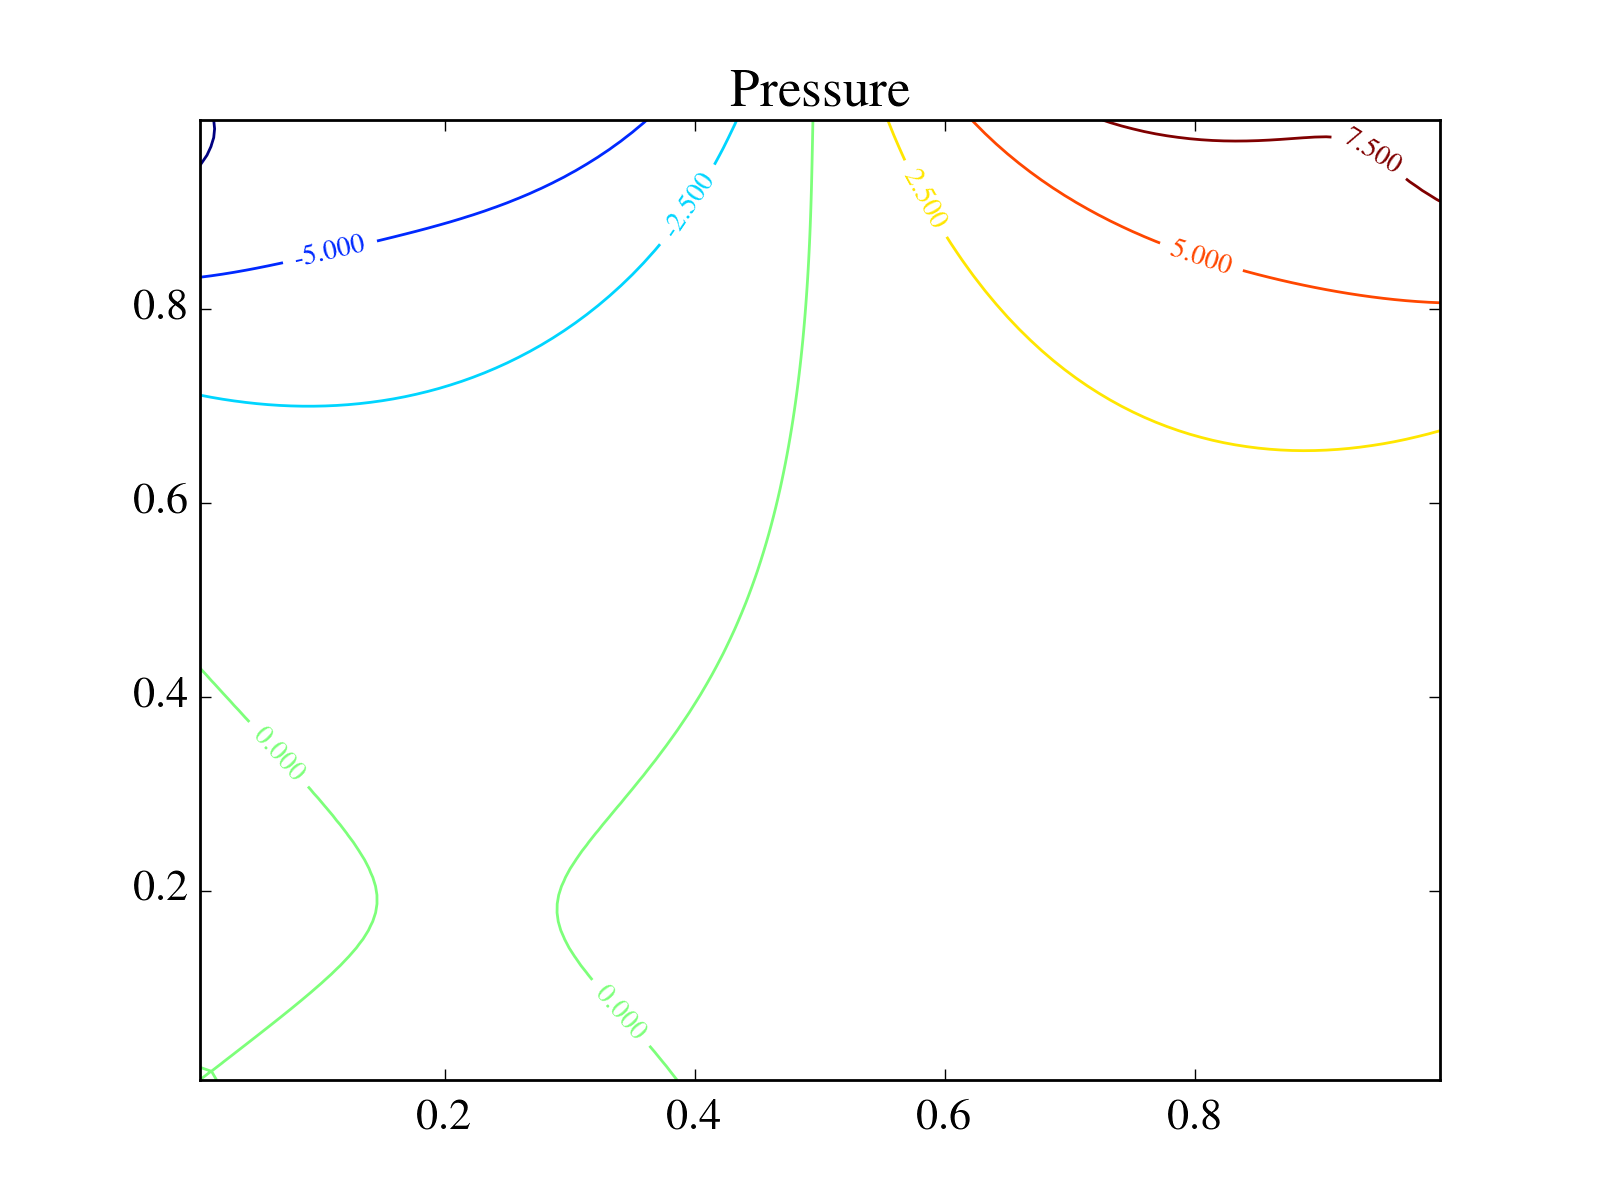
\includegraphics[width=\linewidth]{figures/Re001/n/pressure}
\caption{Contour plot for pressure of the flow in Figure \ref{Re001nVectorField}, $\mathit{Re}=1$, no magnetism. \label{Re001nPressure}}
\end{figure}

\begin{figure}[!t]
\centering
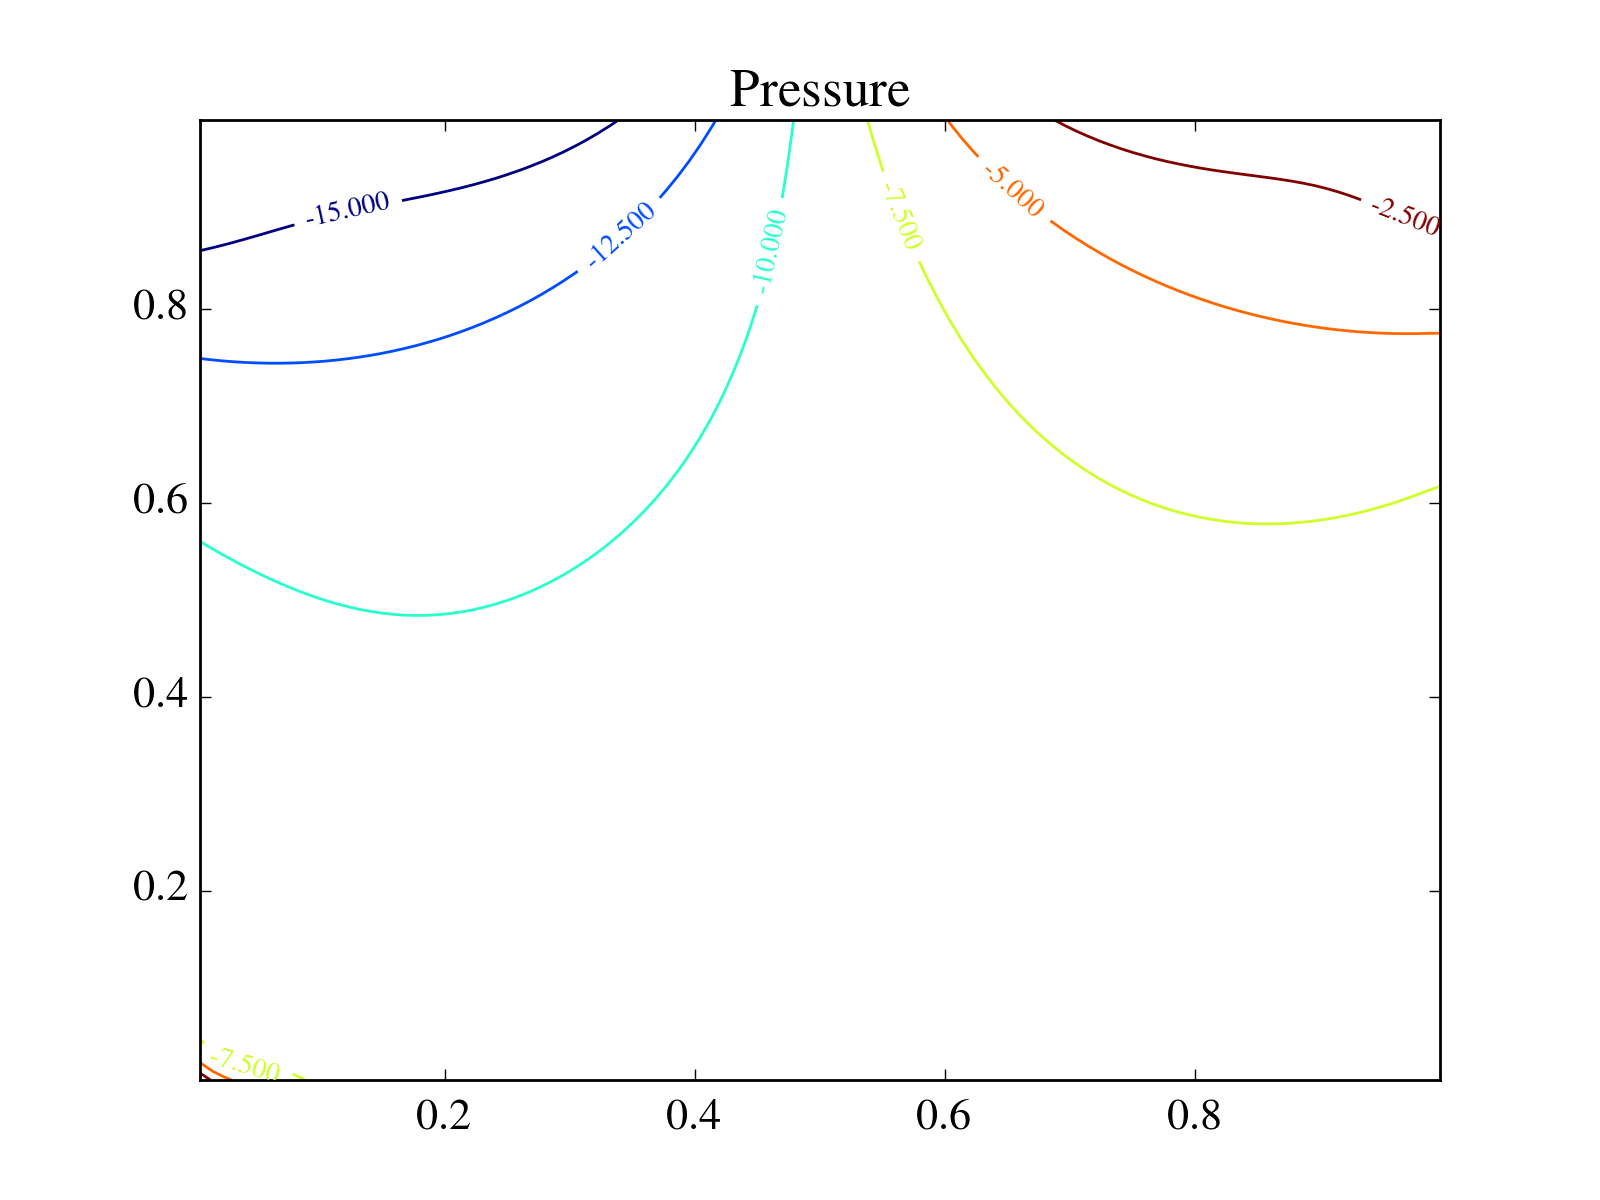
\includegraphics[width=\linewidth]{figures/Re001/w/pressure}
\caption{Contour plot for pressure of the flow in Figure \ref{Re001wVectorField}, $\mathit{Re}=1$, with magnetism\label{Re001wPressure}}
\end{figure}



\begin{figure}[!t]
\centering
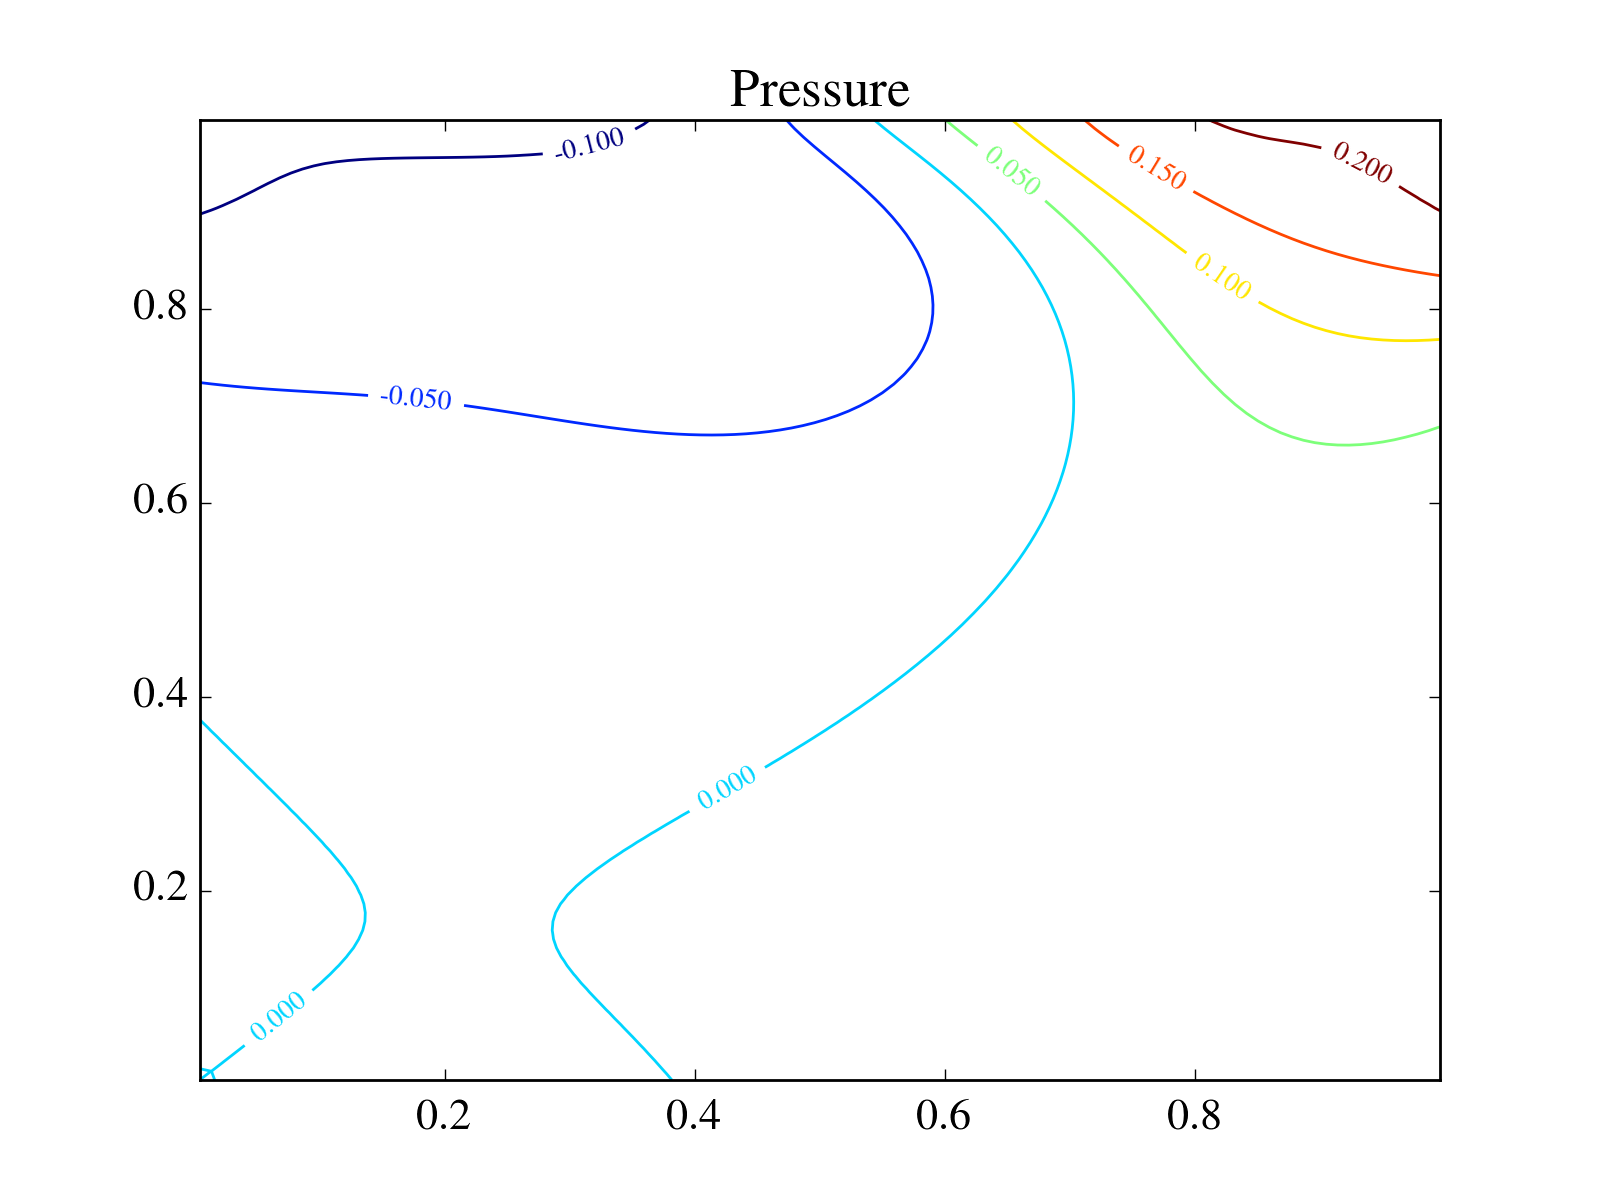
\includegraphics[width=\linewidth]{figures/Re050/n/pressure}
\caption{Contour plot for pressure of the flow in Figure \ref{Re050nVectorField}, $\mathit{Re}=50$, no magnetism\label{Re050nPressure}}
\end{figure}


\begin{figure}[!t]
\centering
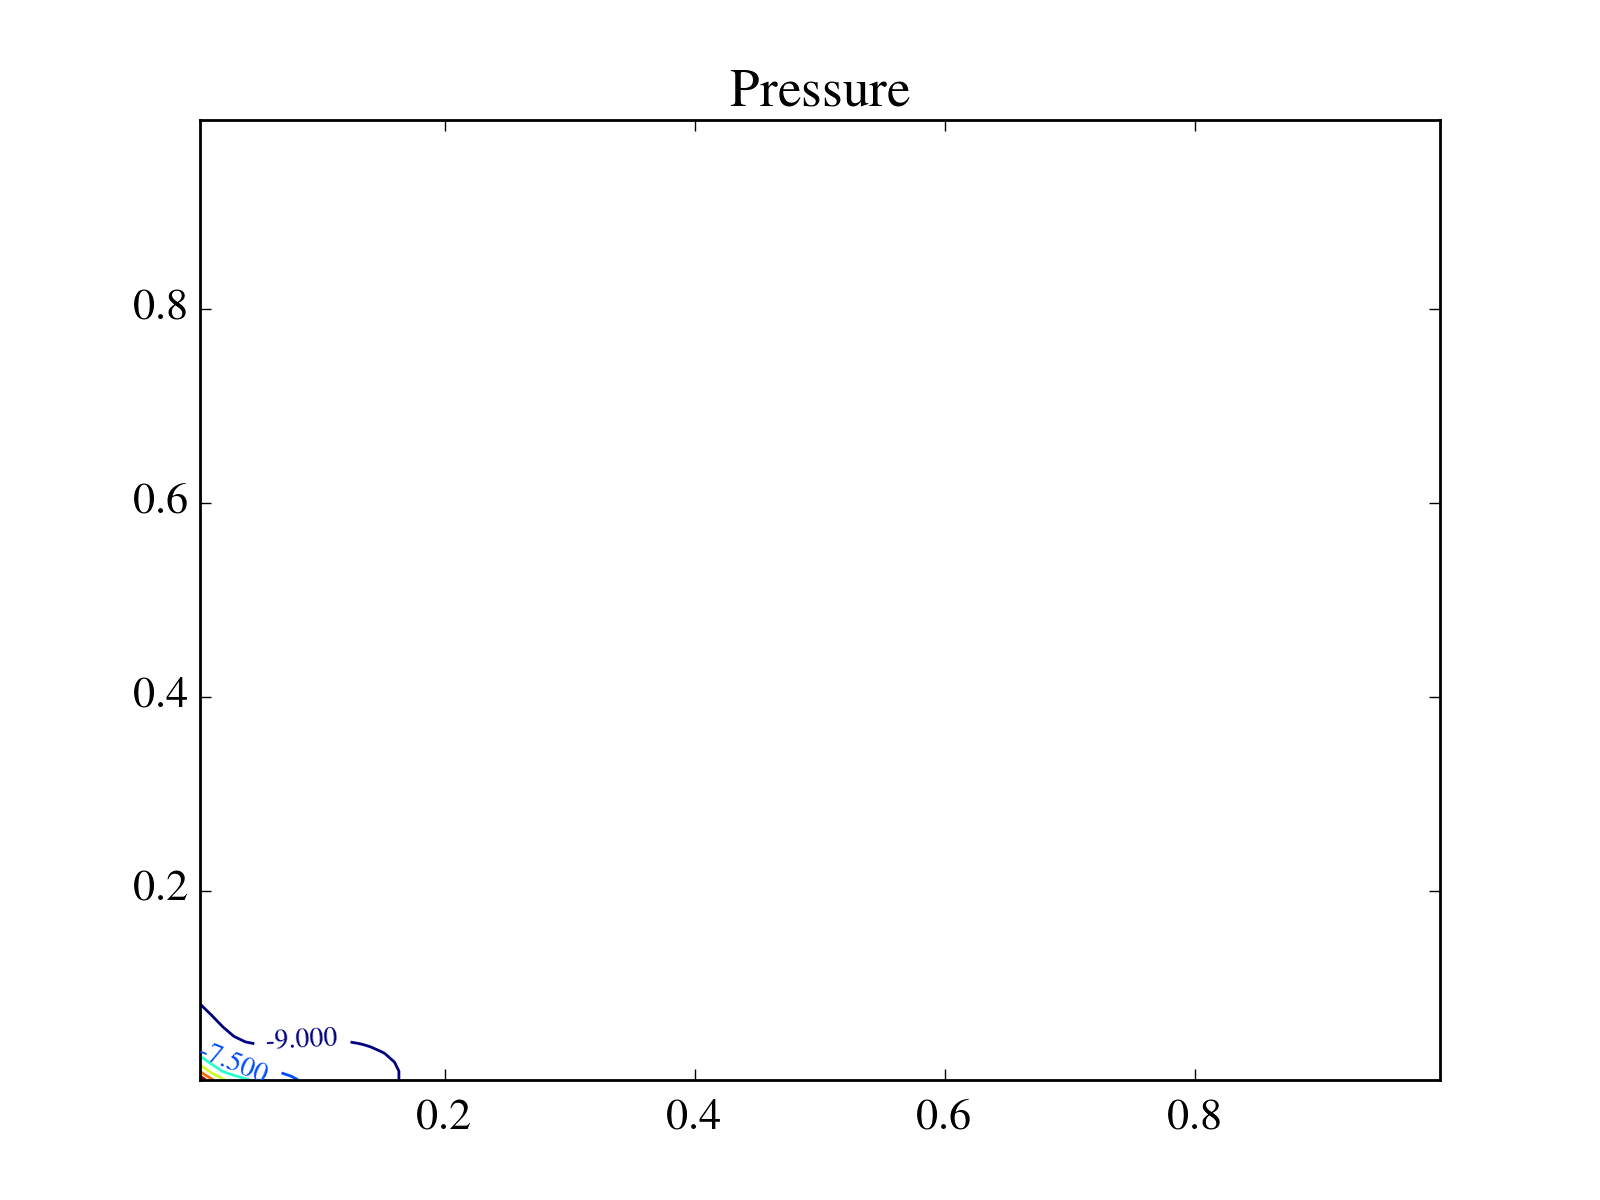
\includegraphics[width=\linewidth]{figures/Re050/w/pressure}
\caption{Contour plot for pressure of the flow in Figure \ref{Re050wVectorField}, $\mathit{Re}=50$, with magnetism \label{Re050wPressure}}
\end{figure}



\begin{figure}[!t]
\centering
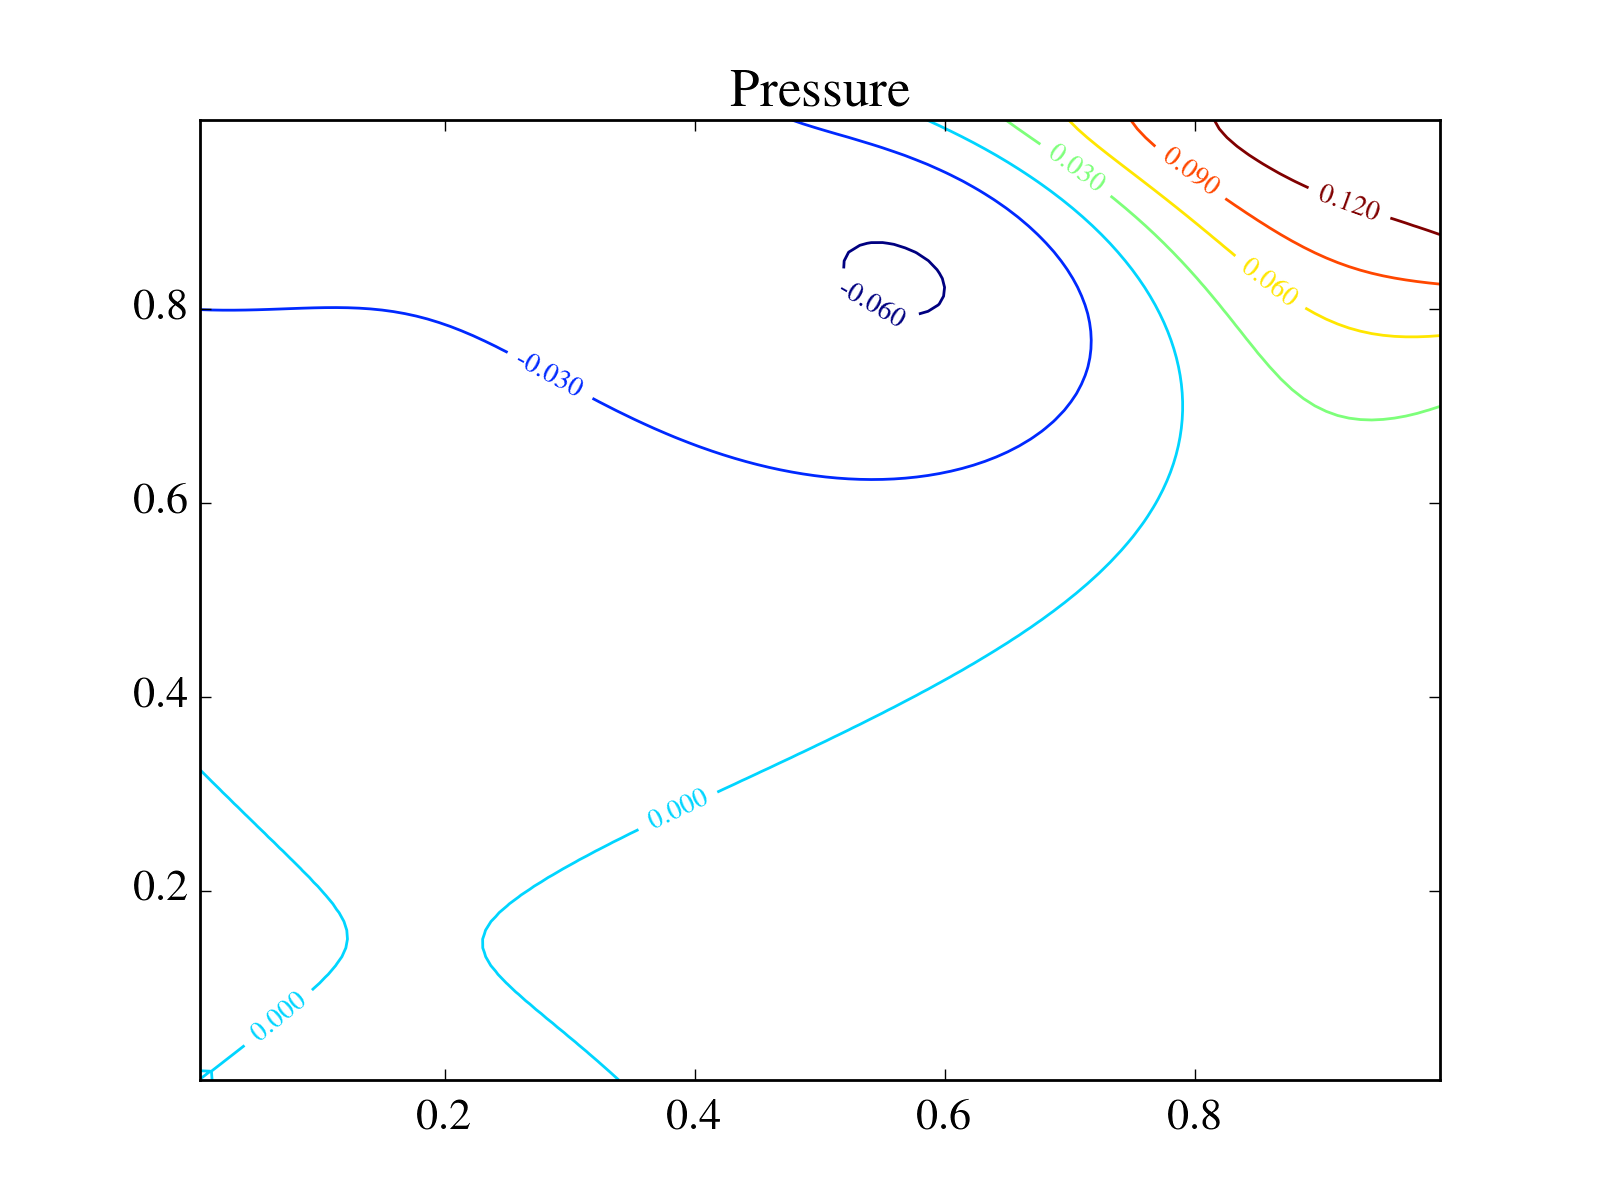
\includegraphics[width=\linewidth]{figures/Re100/n/pressure}
\caption{Contour plot for pressure of the flow in Figure \ref{Re100nVectorField}, $\mathit{Re}=100$, no magnetism\label{Re100nPressure}}
\end{figure}


\begin{figure}[!t]
\centering
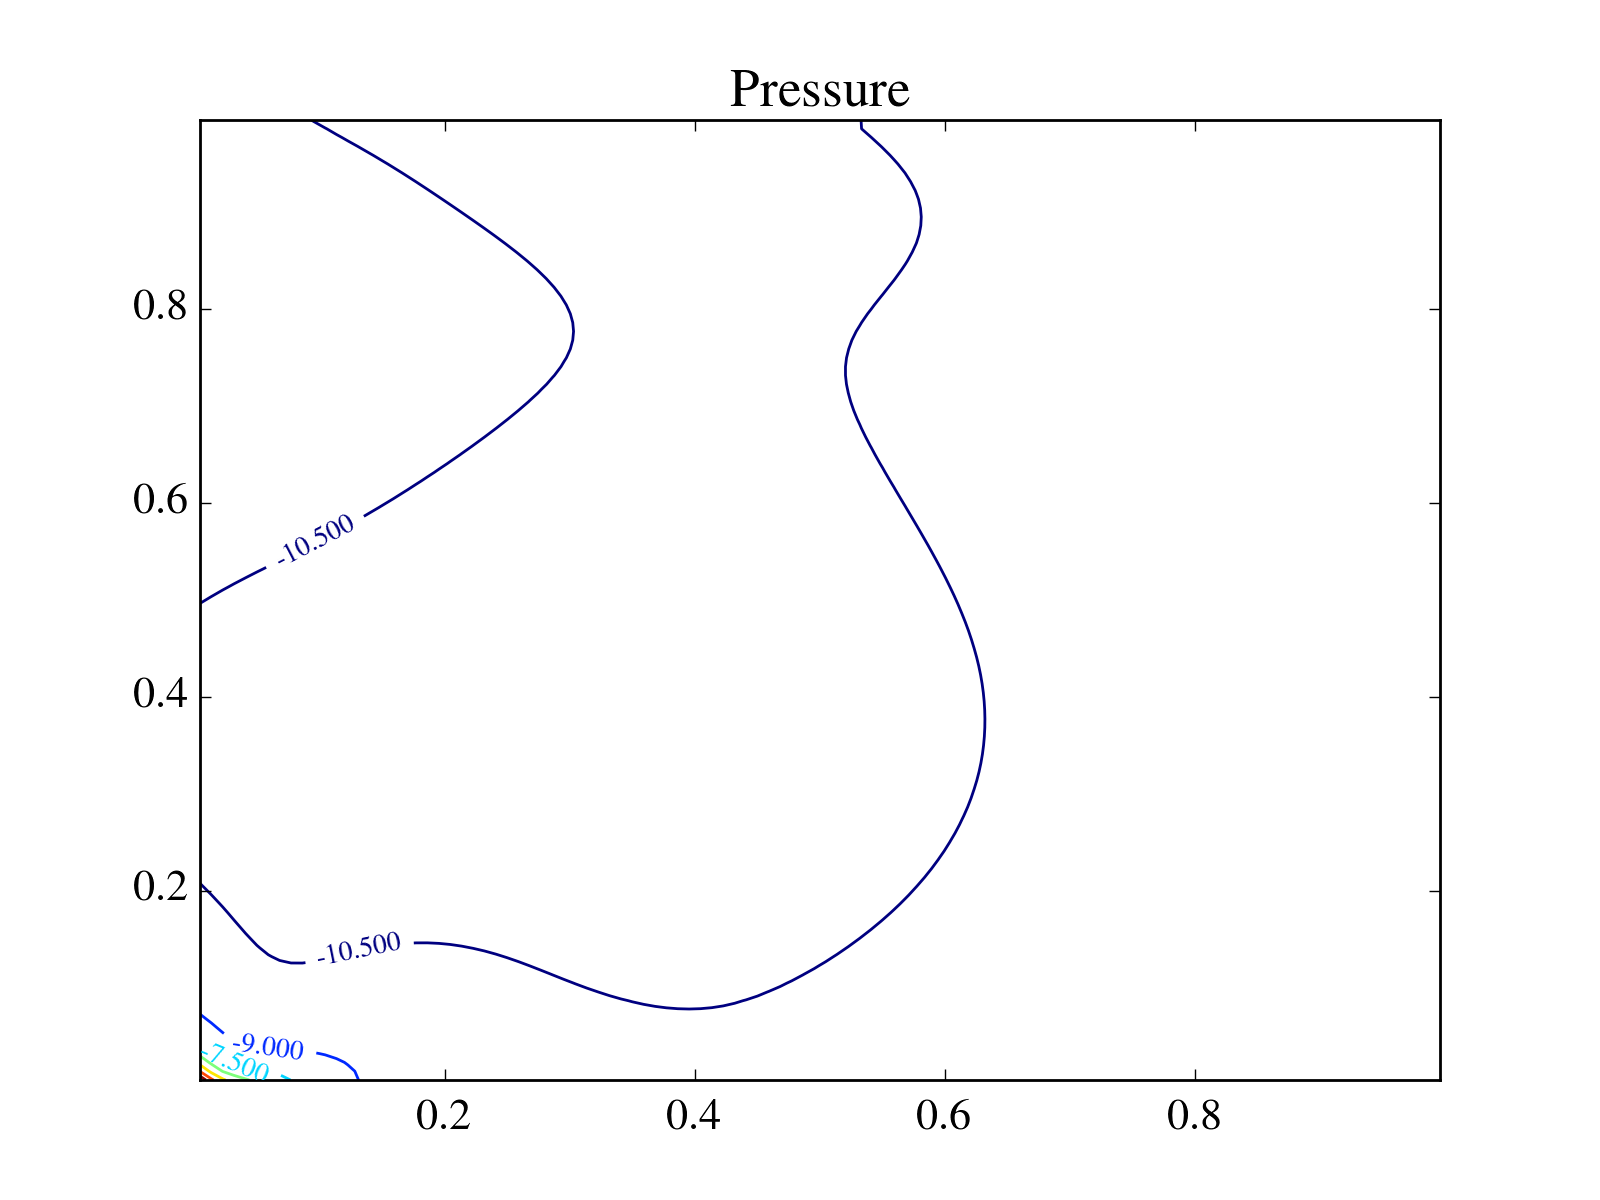
\includegraphics[width=\linewidth]{figures/Re100/w/pressure}
\caption{Contour plot for pressure of the flow in Figure \ref{Re100wVectorField}, $\mathit{Re}=100$, with magnetism \label{Re100wPressure}}
\end{figure}

Regarding the results with no magnetic field, Figures \ref{Re001nVectorField} to \ref{Re100nPressure} present very similar results. Although the Reynolds number changes by a factor of 100, no major changes in the steady state flow were able to be observed. It is noticeable, though, that the flow is more asymmetric and the center of the main vortex shifts to the right as $\mathit{Re}$ increases.

This changes dramatically when a magnetic field is in action. A small vortex already appears in Figure \ref{Re001wVectorField} and just grows larger as the Reynolds number increases up to 100 (Figures \ref{Re050wVectorField} and \ref{Re100wVectorField}). Pressure also changes significantly and a particular concentration of contour lines is observable close to the origin (the magnetic field is applied just a little off the origin) as presented in Figures \ref{Re001wPressure}, \ref{Re050wPressure} and \ref{Re100wPressure}.

Our results are in very good qualitative agreement with the ones presented in \cite{Tzirtzilakis2013}. With this work, we have finalized the step of the construction of the tool that we will use in our next step: a detailed study of different models for the evolution of the magnetization of the ferrofluid in the presence of a flow.


\section{Conclusion}

It is important for the code to be correct, otherwise it is meaningless to analyze the simulation results. The validation step shows that certainly the system is behaving as second order. 

Although not presented in the last sections, it is interesting to observe that one problem that appeared was when physics was disregarded. Trying to apply an arbitrary magnetic field has a good chance of generating results that converge but are incorrect when the governing equations are checked. The results presented comply to the laws that we claim to be following. This is also good evidence of correctness.

This work was a challenge in the aspect that an analytical solution was not available to check against, so it is important to state the importance of the validation step. The results were satisfactory and the tools here coded for exploring magnetic fluids are starting to get usable, specially when compared with the stage of one year ago.


\section{Future work}
The results presented do not include Reynolds greater than 100 because the code is not currently abiding by any upwind scheme. This is something that is planned to be implemented. Also, a different magnetic field will be used, particularly the one of a Neodymium magnet\cite{McCaigClegg}, instead of the magnetic field of a wire\cite{Tzirtzilakis2013}, as used here.

Most importantly, we want to implement the dynamic evolution equations for the magnetization of the ferrofluid that are coupled with the flow field. This will certainly change significantly the dynamics of the flow and will be the subject of our next project.




\section*{Acknowledgments}

Firstly, I thank God for this opportunity. I appreciate professor Yuri Dumaresq for his orientations so that this work could be done. Also, many thanks to CNPq for the scholarship.


\bibliographystyle{plain}
\bibliography{pibic}


\end{document}
